%%%%%%%%%%%%%%%%%%%% Springer SVMult %%%%%%%%%%%%%%%%%%%%%%%%%%%%
\documentclass[graybox]{svmult}

% Springer recommended fonts
\usepackage{mathptmx}       % Times Roman as basic font
\usepackage{helvet}          % Helvetica as sans-serif font
\usepackage{courier}         % Courier as typewriter font
\usepackage{type1cm}        % activate if the above 3 fonts are
                            % not available on your system

% Standard Springer packages
\usepackage{makeidx}         % allows index generation
\usepackage{graphicx}        % standard LaTeX graphics tool
                             % when including figure files
\usepackage{multicol}        % used for the two-column index
\usepackage[bottom]{footmisc}% places footnotes at page bottom

% Additional packages
\usepackage[utf8]{inputenc}
\usepackage[T1]{fontenc}
\usepackage{amsmath,amssymb,amsfonts}
\usepackage{booktabs}
\usepackage{algorithm}
\usepackage{algorithmic}
\usepackage{subcaption}
\usepackage{xcolor}
\usepackage{enumitem}
\usepackage{hyperref}
\usepackage{tikz}
\usepackage{pgfplots}
\pgfplotsset{compat=1.18}
\usetikzlibrary{shapes.geometric, arrows.meta, positioning, calc, fit, backgrounds, patterns, decorations.markings}
\tikzset{
  block/.style={rectangle, draw, fill=blue!8, text width=2.2cm, text centered, minimum height=0.9cm, rounded corners=2pt, font=\small},
  bigblock/.style={rectangle, draw, fill=blue!8, text width=3.0cm, text centered, minimum height=0.9cm, rounded corners=2pt, font=\small},
  decision/.style={diamond, draw, fill=yellow!15, text width=1.6cm, text centered, aspect=2, inner sep=1pt, font=\scriptsize},
  arrow/.style={-{Stealth[length=2.5mm]}, thick},
  darrow/.style={-{Stealth[length=2.5mm]}, thick, dashed},
  neuron/.style={circle, draw, fill=orange!20, minimum size=0.45cm, inner sep=0pt, font=\tiny},
}

\makeindex

% Lightweight theorem-like environment for informal observations.
% svmult already defines `theorem` and `proposition`; we add `observation`
% so our softened formal statements (Section~\ref{sec:formal}) are not
% typeset as full theorems.
\newtheorem{observation}{Observation}

%%%%%%%%%%%%%%%%%%%%%%%%%%%%%%%%%%%%%%%%%%%%%%%%%%%%%%%%%%%%%%%%%%%%%%%%%%%%%%%%%%%%%%%%%

\begin{document}

\pagestyle{empty}

%==============================================================================
\title*{Multi-Solution Search and the Limits of Neural Guidance in Rubik’s Cube Solving}
\titlerunning{Multi-Solution Search and the Limits of Neural Guidance}
%==============================================================================
\author{Akash Chakraborty and Atal Chaudhuri}
\institute{Akash Chakraborty \at Department of Computer Science and Engineering, Sister Nivedita University, Kolkata, \email{akashchakraborty694@gmail.com}
\and Atal Chaudhuri \at Department of Computer Science and Engineering, Sister Nivedita University, Kolkata, \email{atalc23@gmail.com}}

\maketitle
\thispagestyle{empty}

\abstract*{The Rubik’s Cube has roughly $4.3 \times 10^{19}$ reachable states, making brute-force solving impractical. We build on Kociemba’s Two-Phase Algorithm---a well-known near-optimal solver---and investigate three extensions: (i)~\textbf{multi-solution Phase~1 search}, which tries several intermediate paths and keeps the shortest overall solution; (ii)~a \textbf{time-bounded anytime mode} for interactive use; and (iii)~\textbf{neural move ordering} that tries to guide search toward promising moves using learned predictions. On 200 random cubes, multi-solution search cuts the average solution by 0.53~moves and raises the share of $\leq$20-move solutions from 28\% to 57.5\%---a robust and easily deployable improvement. For neural ordering, we report a negative result: although switching from 9 scalar features to 161 binned coordinate features raises raw move-prediction accuracy on native pruning-greedy labels from near-random to 43.9\%, and even after distilling the network into a 576\,KB precomputed lookup table (LUT) that eliminates per-node inference cost, the end-to-end node reduction over plain multi-solution search is only $1.13\times$ and the LUT variant actually solves one fewer cube within the 5~s timeout. We trace this to Kociemba's pruning tables already providing near-optimal move ordering, leaving little room for a learned heuristic to help. A direct headroom measurement on $6{,}000$ walk-sampled search states shows that the oracle move ordering is progressing $65.2\%$ of the time versus $19.6\%$ for Kociemba's default---a gap implying a theoretical $\sim$$10\times$ node-reduction ceiling, not $1\times$---but a multi-output $h$-delta retraining converges to exactly the baseline rate ($20.2\%$), learning the class prior while failing to recover any move-conditional signal. We trace the $1.13\times$ wall to feature resolution rather than baseline strength: the 161-dim binned coordinate features are lossy enough to collapse move-conditional progress within a bin, so lightweight MLP ordering in this regime is not competitive regardless of label quality. All code, data, trained models, and frozen result JSONs are provided for reproducibility.}

\abstract{We extend Kociemba's Two-Phase Rubik's Cube solver with multi-solution Phase~1 search, a time-bounded anytime mode, and neural move ordering. On 200 random cubes, multi-solution search ($K{=}5$) cuts the mean solution by 0.53~moves and raises $\leq$20-move solutions from 28\% to 57.5\%. Neural ordering, even after distillation into a 576\,KB lookup table, yields only $1.13\times$ node reduction---Kociemba's pruning tables already provide near-optimal ordering, leaving little room for learned heuristics. All code, data, and models are provided for reproducibility.}

\textbf{Keywords:} Rubik’s Cube, two-phase algorithm, Kociemba, IDA*, pruning tables, neural heuristics, move ordering, anytime solver

%==============================================================================
\section{Introduction}
\label{sec:intro}
%==============================================================================
\subsection{The Rubik's Cube as a Search Problem}
The Rubik's Cube, invented by Ern\H{o} Rubik in 1974, is one of the most widely studied combinatorial puzzles in computer science~\cite{joyner2008}. A standard $3{\times}3{\times}3$ cube has 26 visible sub-cubes (``cubies''): 8~corners, 12~edges, and 6~face centres. Each corner shows 3 coloured stickers and each edge shows 2, giving 54 stickers in total.

The six faces (Up, Down, Left, Right, Front, Back) can each be turned in three ways---clockwise, counter-clockwise, or a half-turn---yielding 18 possible moves at every step. The number of reachable configurations is
\begin{equation}
|G| = \frac{8! \cdot 3^8 \cdot 12! \cdot 2^{12}}{12} \approx 4.33 \times 10^{19}.
\end{equation}
This enormous state space rules out any brute-force approach.

\subsection{God's Number and Practical Solving}
``God's Number'' is the fewest moves needed to solve any configuration from the worst case. In the \emph{half-turn metric} (HTM), where each quarter-turn or half-turn counts as one move, God's Number is \textbf{20}, proved by Rokicki et al.~\cite{godnumber} in 2010. In other words, every scrambled cube \emph{can} be solved in at most 20~moves---but finding those 20~moves requires searching an astronomically large space.

Kociemba's Two-Phase Algorithm~\cite{kociemba} offers a practical middle ground. It does not guarantee exactly 20~moves for every cube, but it reliably produces 19--22 move solutions in under a second. Although Kociemba's solver is a mature benchmark, two observations motivate this paper. First, its default single-endpoint Phase~1 search accepts the first Phase~1 result it finds, leaving substantial solution-quality headroom unexplored. Second, recent neural-guided search methods such as DeepCubeA~\cite{deepcubea} achieve strong results, but at the cost of days of GPU training, hundreds of thousands of parameters, and per-node inference that does not transfer back to lightweight classical solvers. A practitioner who needs near-optimal solutions on a laptop---for teaching tools, interactive applications, or robotics---is caught between the two extremes.

\subsection{Research Questions and Contributions}
\label{sec:contributions}
This motivates three concrete research questions:
\begin{description}[leftmargin=1.2em, style=nextline]
  \item[\textbf{RQ1}] Can a simple algorithmic extension of Kociemba's solver---exploring multiple Phase~1 endpoints---yield measurable improvements in solution quality without re-training or changing the underlying heuristic?
  \item[\textbf{RQ2}] Does cube-state representation materially affect the accuracy of a learned move predictor attached to a classical IDA* solver, and does any resulting accuracy gain translate into fewer expanded search nodes?
  \item[\textbf{RQ3}] Can the per-node overhead of neural inference be eliminated via lookup-table distillation, and is that sufficient to make learned move ordering competitive with Kociemba's existing pruning-table-based ordering?
\end{description}

\noindent We answer these questions with the following contributions:
\begin{enumerate}[leftmargin=*]
  \item \textbf{Multi-solution Phase~1 search} ($K > 1$): instead of accepting the first intermediate result, the solver explores $K$ alternatives and keeps the shortest combined solution. On 200 random cubes this cuts mean moves by 0.53 (from 20.77 to 20.23) and raises $\leq$20-move solutions from 28\% to 57.5\%, at the cost of an $\approx$8.6$\times$ increase in expanded nodes (RQ1). This is the practical, easily deployable contribution of the paper.
  \item \textbf{Representation affects raw move-prediction accuracy, but not solver node count (negative result).} We train an MLP move predictor under three regimes: (a) 9 scalar features ($\sim$5.6\% proxy-label accuracy, essentially random), (b) 161 binned coordinate features with 100K proxy labels ($\sim$10--13\% validation accuracy, three architectures), and (c) 161 binned coordinate features with 2M pruning-greedy labels (43.9\% native top-1, 64.5\% top-3; depth-stratified from 89.0\% at depth $\leq$5 down to $\approx$30\% at mid-depth). Across all three regimes the end-to-end node reduction over plain $K{=}5$ multi-solution search is within noise ($\leq$1.14$\times$), and the retrained LUT variant actually solves one fewer cube within the 5~s wall-clock budget (RQ2).
  \item \textbf{LUT distillation works as intended, but cannot rescue a heuristic the solver does not need.} Distilling the trained network into a 32K-entry, 576\,KB lookup table drops per-node inference cost to $\approx$1.5\,$\mu$s, eliminating the overhead that Python-native inference imposes. In our 200-cube benchmark this removes the inference-cost barrier but still delivers only a 1.13$\times$ node reduction and \emph{no} wall-clock speedup over non-neural $K{=}5$ search. A direct headroom measurement (Section~\ref{sec:neural-plateau}) shows the gap between the default and oracle move orderings is large ($p_{\text{top}} - p_{\text{lex}} = 0.456$ on $6{,}000$ walk-sampled states, implying a theoretical $\sim$$10\times$ ceiling), and a controlled h-delta retraining experiment shows that our lightweight 161-dim-binned-coordinate predictor cannot reach it---the model converges to the marginal class prior and matches the lexicographic baseline exactly: \emph{the $1.13\times$ wall is a feature-resolution ceiling, not an information-theoretic one} (RQ3).
  \item \textbf{Time-bounded anytime mode} for interactive use, together with an analysis of the ``admissible bound paradox'' (Observation~\ref{thm:bound-paradox}) explaining why a learned lower bound multiplies IDA* iteration cost, an order-statistic argument (Proposition~\ref{prop:order-stat}) for why multi-solution Phase~1 helps, and an empirically calibrated cost model (Observation~\ref{thm:node-reduction}) for when neural move ordering can and cannot pay for itself.
\end{enumerate}

\begin{sloppypar}
\noindent All numbers reported in this paper are taken directly from the frozen artifacts \texttt{results/\allowbreak benchmark\_200\_\allowbreak retrained.json}, \texttt{results/\allowbreak arch\_comp\_\allowbreak replay\_\allowbreak 20260413.json}, and \texttt{results/\allowbreak prun\_greedy\_\allowbreak 2M\_meta.json}, shipped with the code.
\end{sloppypar}

\subsection{Paper Organisation}
Section~\ref{sec:related} reviews prior work. Section~\ref{sec:math} gives the mathematical background. Section~\ref{sec:method} describes our methodology. Sections~\ref{sec:results}--\ref{sec:discussion} present and discuss results. Section~\ref{sec:conclusion} concludes.

%==============================================================================
\section{Related Work}
\label{sec:related}
%==============================================================================

\textbf{Optimal solvers.}
Korf~\cite{korf1997} built the first optimal Rubik's Cube solver using IDA*~\cite{korf1985} with pattern databases~\cite{culberson1998}, later extended to disjoint~\cite{korf2002} and additive~\cite{felner2004} variants. Rokicki et~al.~\cite{godnumber} proved God's Number is 20 using 35~CPU-years of computation. Demaine et~al.~\cite{demaine2018} established worst-case bounds for generalised Rubik's Cubes.

\textbf{Two-phase methods.}
Thistlethwaite~\cite{thistlethwaite1981} introduced nested-subgroup reduction with four phases. Kociemba~\cite{kociemba} simplified this to two phases with coordinate-based pruning tables, dramatically improving speed. Human speedsolving methods like CFOP~\cite{fridrich} use a similar multi-phase strategy but rely on pattern recognition rather than exhaustive search. Our work extends Kociemba's algorithm with multi-solution search and neural ordering.

\textbf{Deep learning for the cube.}
DeepCubeA~\cite{deepcubea} uses deep reinforcement learning with weighted~A* to find optimal solutions in 60\% of cases, but requires $\sim$2 days of GPU training and $\sim$10\,s per solve. Brunetto and Trunda~\cite{brunetto2017} showed that feature representation is critical for distance estimation, consistent with our findings. More recently, Zawalski et~al.~\cite{zawalski2024} systematically compared hierarchical and flat planners on combinatorial puzzles and identified when learned heuristics justify their overhead---a question we answer in the negative for pruning-table-dominated search. Khandelwal et~al.~\cite{khandelwal2024} proposed foundation-model heuristics that generalise across puzzle domains; our LUT distillation is complementary, showing that even a strong learned heuristic must clear the classical baseline's ordering quality to deliver end-to-end gains. More broadly, neural-guided tree search has been transformative in games like Go~\cite{silver2016, silver2017}.

\textbf{Neural heuristics in planning.}
Shen et~al.~\cite{shen2020} showed that small heuristic errors cause exponential node growth in IDA*---the ``heuristic noise'' problem that our Observation~\ref{thm:bound-paradox} formalises. Arfaee et~al.~\cite{arfaee2011} proposed bootstrapped learning of heuristic functions for large state spaces. Ferber et~al.~\cite{ferber2022} demonstrated the importance of domain-specific features for neural heuristics, supporting our finding that binned coordinate features dramatically outperform raw scalars.

\textbf{Positioning.}
Unlike end-to-end learned solvers, we study neural heuristics as \emph{add-ons} to an established classical algorithm, inspired by move-ordering techniques in game-tree search~\cite{schaeffer1989, reinefeld1994}. To our knowledge, we are the first to (i)~demonstrate that neural move ordering \emph{saturates} due to pruning-table dominance in Kociemba's solver, quantifying the precise headroom ($p_{\text{top}} - p_{\text{lex}} = 0.456$) and the feature-resolution ceiling that prevents lightweight models from reaching it; (ii)~distil a trained move predictor into an $O(1)$ lookup table for classical IDA* search; and (iii)~show that multi-solution Phase~1 search alone recovers most of the quality gap that neural methods target, at zero training cost.

%==============================================================================
\section{Mathematical Foundation}
\label{sec:math}
%==============================================================================

\subsection{Coordinate System}
\label{sec:coordinates}

Rather than storing full permutation arrays, the solver encodes each cube state using a small number of \emph{coordinates}---integers that capture the essential structure:

\begin{itemize}[leftmargin=*]
  \item \textbf{Twist} ($0$--$2186$): how the 8 corners are oriented.
  \item \textbf{Flip} ($0$--$2047$): how the 12 edges are oriented.
  \item \textbf{Slice} ($0$--$494$): which 4 of the 12 edge positions hold middle-layer edges.
  \item \textbf{URFtoDLF} and \textbf{URtoDF}: corner and edge permutation coordinates used in Phase~2.
\end{itemize}

The key advantage of coordinates is speed: applying a move just requires looking up $c' = \text{moveTable}[c][m]$, an $O(1)$ table lookup.

\subsection{How the Two-Phase Algorithm Works}
\label{sec:two-phase}

The algorithm solves the cube in two stages (Fig.~\ref{fig:pipeline}):

\textbf{Phase~1} searches for a sequence of moves that brings the cube from its scrambled state into a special subgroup
\begin{equation}
G_1 = \langle U, D, L^2, R^2, F^2, B^2 \rangle.
\end{equation}
A cube is in $G_1$ when all edges are correctly oriented (flip $= 0$), all corners are correctly oriented (twist $= 0$), and the four middle-layer edges are in middle-layer positions (slice $= 0$). Phase~1 uses all 18 moves.

\textbf{Phase~2} takes the cube from the $G_1$ state to the solved state (the identity). Only 10 moves are allowed (the generators of $G_1$), so the effective branching factor drops from 18 to 10 and stronger pruning tables apply. Phase~2 is typically much faster than Phase~1.

Both phases use \textbf{IDA*} (Iterative Deepening A*)~\cite{korf1985}, a memory-efficient extension of A*~\cite{hart1968}. IDA* performs repeated depth-first searches with an increasing cost limit. At each node, a heuristic lower bound $h$~\cite{pearl1984} (read from precomputed \emph{pruning tables}) estimates the remaining moves. If the current depth $g$ plus $h$ exceeds the limit, the branch is pruned. The critical property for our analysis: the number of nodes grows \emph{exponentially} with the depth limit, so adding even one extra level of search multiplies the work by $\sim$13.

\subsection{Pruning Tables}
\label{sec:pruning}
Pruning tables store the minimum moves needed to reach the target (the $G_1$ subgroup in Phase~1, or the identity in Phase~2) from each coordinate value. They are built once by backward breadth-first search and cached on disk ($\sim$20\,MB). The heuristic at each node is the maximum of two independent lower bounds (e.g., Slice--Twist and Slice--Flip for Phase~1), which tightens the estimate while remaining admissible.

\begin{figure}[!t]
\centering
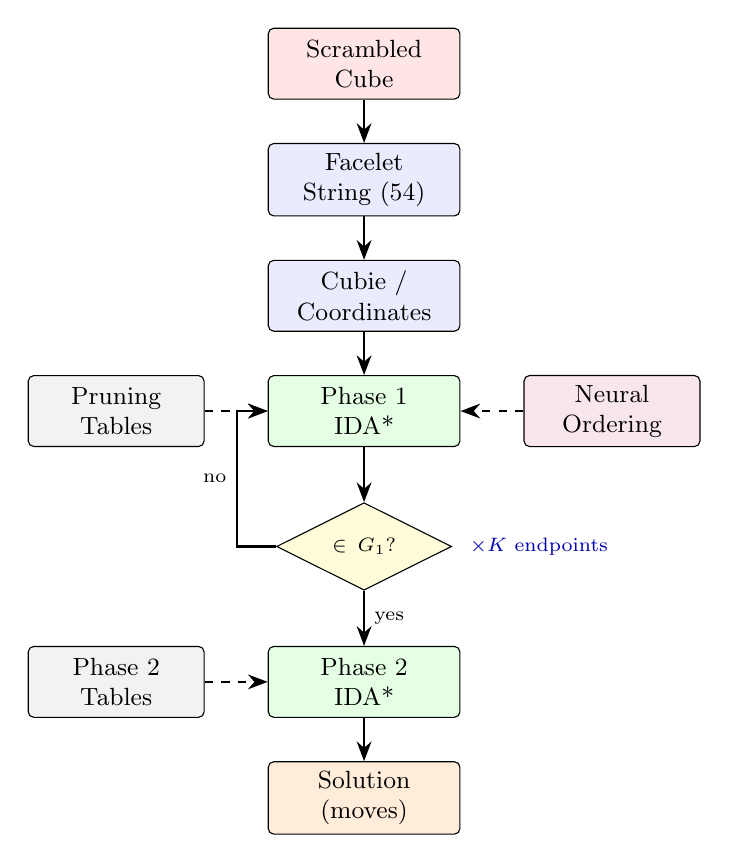
\begin{tikzpicture}[node distance=0.55cm and 0.4cm, >=Stealth, font=\small]
  \node[block, fill=red!10] (input) {Scrambled\\Cube};
  \node[block, below=of input] (facelet) {Facelet\\String (54)};
  \node[block, below=of facelet] (cubie) {Cubie /\\Coordinates};
  \node[block, fill=green!10, below=of cubie] (phase1) {Phase~1\\IDA*};
  \node[decision, below=0.7cm of phase1] (g1check) {$\in G_1$?};
  \node[block, fill=green!10, below=0.7cm of g1check] (phase2) {Phase~2\\IDA*};
  \node[block, fill=orange!15, below=of phase2] (solution) {Solution\\(moves)};
  \node[block, fill=purple!10, text width=2.0cm, right=0.8cm of phase1] (neural) {Neural\\Ordering};
  \node[block, fill=gray!10, text width=2.0cm, left=0.8cm of phase1] (prune1) {Pruning\\Tables};
  \node[block, fill=gray!10, text width=2.0cm, left=0.8cm of phase2] (prune2) {Phase~2\\Tables};
  \draw[arrow] (input) -- (facelet);
  \draw[arrow] (facelet) -- (cubie);
  \draw[arrow] (cubie) -- (phase1);
  \draw[arrow] (phase1) -- (g1check);
  \draw[arrow] (g1check) -- node[right, font=\scriptsize] {yes} (phase2);
  \draw[arrow] (g1check.west) -- ++(-0.5,0) |- node[left, pos=0.25, font=\scriptsize] {no} (phase1.west);
  \draw[arrow] (phase2) -- (solution);
  \draw[darrow] (neural) -- (phase1);
  \draw[darrow] (prune1) -- (phase1);
  \draw[darrow] (prune2) -- (phase2);
  \node[font=\scriptsize, text=blue!70!black, right=0.1cm of g1check.east] {$\times K$ endpoints};
\end{tikzpicture}
\caption{Solver pipeline. The scrambled cube is converted to coordinates, then Phase~1 searches for states in subgroup $G_1$ (optionally guided by neural ordering). Phase~2 completes the solve. With $K > 1$, multiple Phase~1 endpoints are tried and the shortest overall solution is kept.}
\label{fig:pipeline}
\end{figure}

\subsection{Consecutive Move Pruning}
At each node the solver considers all 18 moves, but two simple rules eliminate redundant branches without losing solutions: (1)~never apply two moves of the \emph{same} face in a row (e.g., $U$ then $U'$ is just $U2$ or the identity), and (2)~for opposite faces that commute ($U/D$, $L/R$, $F/B$), impose a fixed ordering to avoid duplicates ($UD = DU$). These rules reduce the average branching factor from 18 to about 13.35---a $\sim$500$\times$ reduction in tree size at depth 20.

\subsection{Formal Results}
\label{sec:formal}

\begin{sloppypar}
We now state three results that combine analytical reasoning with empirical calibration---one observation about learned lower bounds in IDA*, one order-statistic proposition about multi-solution search, and one cost model for learned move ordering. Each statement is accompanied by a derivation sketch and empirical verification; they do not claim the generality of formal theorems but are predictive in our setting, and their quantitative predictions are confirmed by our experiments (Sections~\ref{sec:results}--\ref{sec:discussion}).
\end{sloppypar}

\begin{observation}[Admissible Bound Paradox]
\label{thm:bound-paradox}
Let $h^*$ be the optimal admissible heuristic for IDA*, and let $\hat{h} = h^* + \epsilon$ be a learned heuristic that is \emph{not} guaranteed admissible, overestimating on some states by up to $\epsilon > 0$ moves. Then, in the worst case, IDA* with $\hat{h}$ expands on the order of $b_{\mathrm{eff}}^{\lceil\epsilon\rceil}$ times more nodes than IDA* with $h^*$, because each additional IDA* iteration costs a factor $b_{\mathrm{eff}}$ more than the previous one.
\end{observation}

\textbf{Sketch.} IDA* expands $O(b_{\mathrm{eff}}^d)$ nodes at threshold $d$. An inadmissible heuristic can prune parts of an optimal-length path at threshold $d^*$, forcing the search to deepen to $d^* + \lceil\epsilon\rceil$. The final iteration alone costs $O(b_{\mathrm{eff}}^{d^* + \lceil\epsilon\rceil})$, giving the claimed factor. This is a worst-case statement and relies on $\epsilon$ being triggered somewhere along an optimal path; it is not a pointwise guarantee.

\textbf{Why this matters.} The tempting way to use a learned value network in IDA* is as a tighter (non-admissible) lower bound. The observation above is our reason for \emph{not} doing that, and for using neural predictions only as a move-ordering hint, which preserves admissibility.

\begin{proposition}[Multi-Solution Order-Statistic Bound]
\label{prop:order-stat}
If $K$ Phase~1 endpoints yield solution lengths modeled as i.i.d.\ samples with mean $\mu$ and standard deviation $\sigma$, the expected length of the minimum is approximately $\mu - \sigma \cdot c_K$~\cite{david2003}, where $c_K > 0$ grows slowly with $K$ (for $K{=}5$, $c_K \approx 1.16$).
\end{proposition}

\noindent In plain terms: trying multiple Phase~1 paths and keeping the best gives shorter solutions on average, with diminishing returns as $K$ grows. The i.i.d.\ assumption is optimistic (successive endpoints share structure), so in practice the observed gain is smaller than this bound predicts.

\begin{observation}[Node Reduction Ceiling for Move Ordering]
\label{thm:node-reduction}
\begin{sloppypar}
Consider an idealised model in which, at each node, a learned predictor places the locally best move first with probability $p$, independently across nodes. If the baseline move order is already close to optimal---as is the case when Kociemba's pruning tables induce an ordering that is correct with probability $p_0$---then the extra multiplicative node reduction available to a learned ordering with success rate $p$ is at most on the order of $(1 - (p - p_0)(1 - 1/b))^d$, with $b$ the branching factor and $d$ the search depth. When $p \approx p_0$, the ceiling is $\approx 1$: no meaningful reduction.
\end{sloppypar}
\end{observation}

\textbf{Caveat.} The textbook formula for node reduction from move ordering assumes the \emph{baseline} is random. In IDA* with strong pruning tables the baseline is far from random, so the relevant quantity is the gap between Kociemba's fixed lexicographic move ordering and the true optimal ordering---not $1/b$. We measure this gap directly in Section~\ref{sec:neural-plateau}: on $6{,}000$ walk-sampled Phase~1 states the rate at which the default first-legal child is progressing is $p_{\text{lex}} = 0.196$, while the rate for the minimum-$h$ child is $p_{\text{top}} = 0.652$. Plugging these into the expression above with $b \approx 13.5$ and $d \approx 7$ implies a theoretical node-reduction ceiling on the order of $10\times$---meaningful headroom, not $1\times$. Our empirical $1.13{\times}$--$1.14{\times}$ (Section~\ref{sec:results}) is therefore not an information-theoretic limit; Section~\ref{sec:neural-plateau} traces it to \emph{feature resolution}: the 161-dim binned coordinate features are (near-)sufficient for state-level quantities such as $h$ but lossy enough that no MLP on top of them can learn move-conditional $\Delta h$ beyond the marginal class prior. This prediction---that the ceiling is a property of the feature representation, not of the search problem---is confirmed by two independent experiments: the h-delta retraining (Section~\ref{sec:neural-plateau}) converges to the class prior, and the oracle \texttt{h\_sort} experiment (Section~\ref{sec:h-sort}) achieves a $1.66\times$ node reduction using full pruning-table access, validating that the headroom is real.

\begin{quote}
\textbf{Takeaway.} \emph{Prediction accuracy alone is not a sufficient metric for evaluating heuristic usefulness in search.} What matters is the gap between the learned ordering and the existing baseline ordering along the search frontier actually visited by the solver---not the top-1 accuracy on a held-out validation set.
\end{quote}

%==============================================================================
\section{Methodology and Implementation}
\label{sec:method}
%==============================================================================

\subsection{System Overview}
The solver, built on the \texttt{kociemba} Python package~\cite{muodov}, uses two representations: a \textbf{facelet string} (54 characters, one per sticker) for input/output, and \textbf{coordinates} for search. Translation happens once per solve. Moves are applied via precomputed table lookups, making each move $O(1)$.

\subsection{User Flow: 3D Cube State Input}
\label{sec:user-flow}

The application exposes an interactive Matplotlib-based 3D cube with a 2D unfolded net and a colour palette. With the physical cube held in a fixed orientation (white top, blue front), the user cycles through faces via click or \texttt{Tab}\,/\,\texttt{Shift+Tab} (a \texttt{G}-toggled guided mode walks first-time users sticker-by-sticker), paints the eight non-centre stickers per face via click-then-palette or the \texttt{1}--\texttt{6} keyboard shortcut (centres are locked to prevent a common input error), and sees both views update in real time. Pressing \texttt{Enter} validates the colour histogram (nine stickers per colour), converts the grid to a 54-character facelet string, and invokes the two-phase solver. \texttt{R} resets to the solved state; individual stickers can be repainted at any time. This replaces the earlier camera-based pipeline, removing lighting- and calibration-dependent errors.

\subsection{Multi-Solution Phase~1 Search}
\label{sec:multi-phase1}

The baseline Kociemba solver returns the \emph{first} Phase~1 solution and runs Phase~2 once, but different Phase~1 paths reach different points in $G_1$ and the Phase~2 distance from each varies. Our extension is a \textbf{multi-endpoint strategy exploiting Phase~2 variance}: parameter $K$ instructs the solver to find up to $K$ Phase~1 endpoints, run Phase~2 from each, and keep the shortest overall solution. Proposition~\ref{prop:order-stat} gives the expected minimum as $\mu - \sigma c_K$ ($c_5 \approx 1.16$), so $K$ controls a principled trade-off between variance reduction and extra search work. $K{=}1$ recovers baseline behaviour; $K{>}1$ trades compute for shorter solutions (Algorithm~\ref{alg:multi-phase1}, Fig.~\ref{fig:multi-solution}).

\begin{algorithm}[t]
\caption{Multi-Solution Phase~1 IDA*}
\label{alg:multi-phase1}
\begin{algorithmic}[1]
\REQUIRE Cube state $s_0$, max solutions $K$, time budget $T$
\ENSURE Best solution found
\STATE $d_{\text{limit}} \gets h_1(s_0)$
\STATE $\text{best} \gets \text{None}$; $\text{best\_len} \gets \infty$; $\text{count} \gets 0$
\WHILE{$\text{count} < K$ \AND elapsed $< T$}
  \STATE $t \gets$ \textsc{DFS-Phase1}($s_0$, $0$, $d_{\text{limit}}$)
  \IF{$t = \text{FOUND}$}
    \STATE \textbf{continue}
  \ELSIF{$t = \infty$}
    \STATE \textbf{break} \COMMENT{No more solutions}
  \ELSE
    \STATE $d_{\text{limit}} \gets t$ \COMMENT{Raise threshold}
  \ENDIF
\ENDWHILE
\STATE \textbf{return} best
\end{algorithmic}
\end{algorithm}

\begin{figure}[!t]
\centering
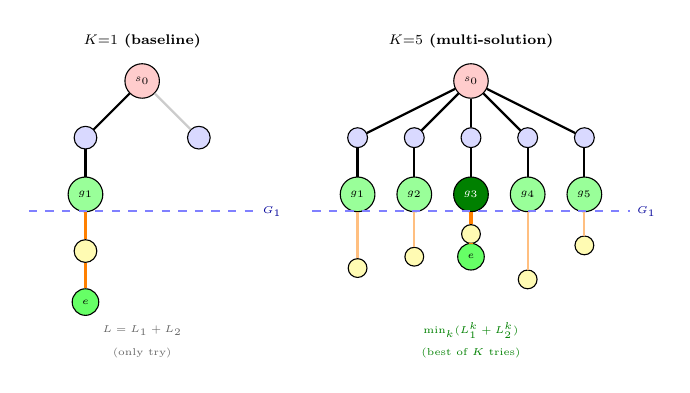
\begin{tikzpicture}[font=\small, scale=0.72, every node/.style={scale=0.72}]
  % K=1 tree (left)
  \node[font=\scriptsize\bfseries] at (-2.8, 3.2) {$K{=}1$ (baseline)};
  \node[circle, draw, fill=red!20, minimum size=5mm, font=\tiny] (r1) at (-2.8, 2.5) {$s_0$};
  \node[circle, draw, fill=blue!15, minimum size=4mm, font=\tiny] (a1) at (-3.8, 1.5) {};
  \node[circle, draw, fill=blue!15, minimum size=4mm, font=\tiny] (a2) at (-1.8, 1.5) {};
  \node[circle, draw, fill=green!40, minimum size=4mm, font=\tiny] (g1) at (-3.8, 0.5) {$g_1$};
  \draw[thick] (r1) -- (a1);
  \draw[thick, gray!40] (r1) -- (a2);
  \draw[thick] (a1) -- (g1);
  \draw[dashed, blue!50, thick] (-4.8, 0.2) -- (-0.8, 0.2) node[right, font=\tiny, text=blue!60!black] {$G_1$};
  \node[circle, draw, fill=yellow!30, minimum size=4mm, font=\tiny] (p2a) at (-3.8, -0.5) {};
  \node[circle, draw, fill=green!60, minimum size=4mm, font=\tiny] (sol1) at (-3.8, -1.4) {$e$};
  \draw[thick, orange] (g1) -- (p2a) -- (sol1);
  \node[font=\tiny, text=black!60] at (-2.8, -1.9) {$L = L_1 + L_2$};
  \node[font=\tiny, text=black!60] at (-2.8, -2.3) {(only try)};
  % K=5 tree (right)
  \node[font=\scriptsize\bfseries] at (3.0, 3.2) {$K{=}5$ (multi-solution)};
  \node[circle, draw, fill=red!20, minimum size=5mm, font=\tiny] (r2) at (3.0, 2.5) {$s_0$};
  \foreach \i/\x in {1/1.0, 2/2.0, 3/3.0, 4/4.0, 5/5.0} {
    \node[circle, draw, fill=blue!15, minimum size=3.5mm] (b\i) at (\x, 1.5) {};
    \draw[thick] (r2) -- (b\i);
  }
  \node[circle, draw, fill=green!40, minimum size=3.5mm, font=\tiny] (e1) at (1.0, 0.5) {$g_1$};
  \node[circle, draw, fill=green!40, minimum size=3.5mm, font=\tiny] (e2) at (2.0, 0.5) {$g_2$};
  \node[circle, draw, fill=green!50!black, minimum size=3.5mm, font=\tiny, text=white] (e3) at (3.0, 0.5) {$g_3$};
  \node[circle, draw, fill=green!40, minimum size=3.5mm, font=\tiny] (e4) at (4.0, 0.5) {$g_4$};
  \node[circle, draw, fill=green!40, minimum size=3.5mm, font=\tiny] (e5) at (5.0, 0.5) {$g_5$};
  \foreach \i in {1,...,5} { \draw[thick] (b\i) -- (e\i); }
  \draw[dashed, blue!50, thick] (0.2, 0.2) -- (5.8, 0.2) node[right, font=\tiny, text=blue!60!black] {$G_1$};
  \foreach \i/\len in {1/5, 2/4, 3/2, 4/6, 5/3} {
    \pgfmathsetmacro{\ybot}{0.2 - \len*0.2}
    \node[circle, draw, fill=yellow!30, minimum size=2.5mm] (p\i) at (\i, \ybot) {};
    \draw[thick, orange!50] (e\i) -- (p\i);
  }
  \draw[thick, orange, line width=1.5pt] (e3) -- (p3);
  \node[circle, draw, fill=green!60, minimum size=3.5mm, font=\tiny] (best) at (3.0, -0.6) {$e$};
  \draw[thick, orange, line width=1.5pt] (p3) -- (best);
  \node[font=\tiny, text=green!50!black] at (3.0, -1.9) {$\min_k(L_1^k + L_2^k)$};
  \node[font=\tiny, text=green!50!black] at (3.0, -2.3) {(best of $K$ tries)};
\end{tikzpicture}
\caption{Multi-solution Phase~1. Left: $K{=}1$ finds one $G_1$ endpoint and accepts whatever Phase~2 gives. Right: $K{=}5$ finds five endpoints, runs Phase~2 from each, and returns the shortest total (dark green, $g_3$). Mean improvement on the canonical seed-42 run: $-0.53$ moves ($p < 10^{-20}$, $d_z = 0.79$).}
\label{fig:multi-solution}
\end{figure}

\subsection{Time-Bounded Anytime Mode}
\label{sec:anytime}

For interactive applications, unbounded solve time is unacceptable. We add an optional time budget $T$ (e.g., 0.5\,s). Before each Phase~1 iteration the solver checks the clock; if time is up and at least one solution exists, it returns the best solution found so far. The quality is monotonically non-decreasing: once a solution is found (typically within 100\,ms), it can only be improved or kept, never worsened.

\subsection{Neural Move Ordering}
\label{sec:neural-strategies}

At each search node, instead of trying the 18 moves in a fixed order, a neural network ranks them by predicted promise and the solver tries those first. IDA* still explores every non-pruned child regardless of order, so the set of solutions is unchanged---only the order in which they are reached. The alternative---using the prediction as a tighter lower bound---runs straight into Observation~\ref{thm:bound-paradox}: any overestimate forces extra IDA* iterations at exponential cost, producing the order-of-magnitude slowdowns we observed in preliminary experiments. We therefore use neural predictions only as move-ordering hints. Three integration strategies---(A)~\emph{always order}, (B)~\emph{probabilistic} with probability $p$, and (C)~\emph{depth-cutoff} at depths $\leq D_{\mathrm{cut}}$---all leave the pruning bound unchanged.

\subsection{Neural Network Architecture}
\label{sec:neural-arch}

We train two models:

\textbf{Move predictor} ($\pi_\theta$): an MLP (Fig.~\ref{fig:mlp-arch}) mapping the cube state to a distribution over 18 moves ($324 \to 256 \to 128 \to 64 \to 18$, ReLU activations, softmax output). The input is a 54-sticker one-hot encoding (54~positions $\times$ 6~colours = 324 dimensions) or a 161-dimensional coordinate feature vector (described in Section~\ref{sec:coord-features}).

\textbf{Value predictor} ($v_\phi$): an MLP estimating moves-to-solve ($324 \to 512 \to 256 \to 128 \to 1$). Used only to analyse the admissible bound paradox; \emph{not} used in any strategy.

\begin{figure}[!t]
\centering
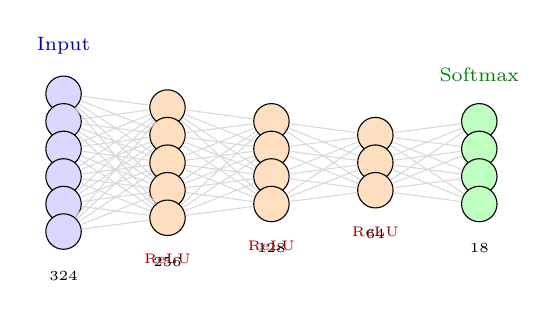
\begin{tikzpicture}[x=1.1cm, y=0.35cm]
  \def\layerA{6}
  \def\layerB{5}
  \def\layerC{4}
  \def\layerD{3}
  \def\layerE{4}
  \foreach \i in {1,...,\layerA} {
    \node[neuron, fill=blue!15] (i\i) at (0, {-\i + (\layerA+1)/2}) {};
  }
  \node[font=\tiny, below=0.15cm of i\layerA] {324};
  \node[font=\scriptsize, above=0.15cm of i1, text=blue!70!black] {Input};
  \foreach \i in {1,...,\layerB} {
    \node[neuron, fill=orange!25] (h1\i) at (1.2, {-\i + (\layerB+1)/2}) {};
  }
  \node[font=\tiny, below=0.15cm of h1\layerB] {256};
  \foreach \i in {1,...,\layerC} {
    \node[neuron, fill=orange!25] (h2\i) at (2.4, {-\i + (\layerC+1)/2}) {};
  }
  \node[font=\tiny, below=0.15cm of h2\layerC] {128};
  \foreach \i in {1,...,\layerD} {
    \node[neuron, fill=orange!25] (h3\i) at (3.6, {-\i + (\layerD+1)/2}) {};
  }
  \node[font=\tiny, below=0.15cm of h3\layerD] {64};
  \foreach \i in {1,...,\layerE} {
    \node[neuron, fill=green!25] (o\i) at (4.8, {-\i + (\layerE+1)/2}) {};
  }
  \node[font=\tiny, below=0.15cm of o\layerE] {18};
  \node[font=\scriptsize, above=0.15cm of o1, text=green!50!black] {Softmax};
  \foreach \i in {1,...,\layerA} {
    \foreach \j in {1,...,\layerB} {
      \draw[gray!30, thin] (i\i) -- (h1\j);
    }
  }
  \foreach \i in {1,...,\layerB} {
    \foreach \j in {1,...,\layerC} {
      \draw[gray!30, thin] (h1\i) -- (h2\j);
    }
  }
  \foreach \i in {1,...,\layerC} {
    \foreach \j in {1,...,\layerD} {
      \draw[gray!30, thin] (h2\i) -- (h3\j);
    }
  }
  \foreach \i in {1,...,\layerD} {
    \foreach \j in {1,...,\layerE} {
      \draw[gray!30, thin] (h3\i) -- (o\j);
    }
  }
  \node[font=\tiny, text=red!60!black] at (1.2, -3.5) {ReLU};
  \node[font=\tiny, text=red!60!black] at (2.4, -3.0) {ReLU};
  \node[font=\tiny, text=red!60!black] at (3.6, -2.5) {ReLU};
\end{tikzpicture}
\caption{Move predictor MLP. The one-hot encoding (324~dims) or coordinate features (161~dims) pass through three hidden layers. The 18-way softmax output gives a distribution over moves for ordering. Parameter counts depend on the input variant: the 324-dim one-hot gives $\approx$125K parameters; the 161-dim coordinate variant used throughout Section~\ref{sec:coord-features} and Table~\ref{tab:arch-comparison} gives 83,794 (``84K'') parameters for the same hidden sizes.}
\label{fig:mlp-arch}
\end{figure}

\textbf{Training.} We report three training regimes used in different experiments.
\begin{enumerate}[leftmargin=*]
\begin{sloppypar}
  \item \emph{Scalar baseline}: 9-dimensional scalar coordinates, $\sim$50K cubes with proxy labels (the reverse of the last scramble move), 30 epochs, batch size 64, Adam~\cite{kingma2015} ($\text{lr}=10^{-3}$). Validation accuracy $\approx$5.6\%.
  \item \emph{Coordinate proxy-label run} (used for the architecture comparison in Table~\ref{tab:arch-comparison}, frozen at \texttt{results/\allowbreak arch\_comp\_replay\_20260413.json}): 161-dim binned coordinate features, 100K cubes, proxy labels, seed 42, 100 epochs per architecture. Three architectures (MLP-3, MLP-4 Wide, MLP-5 Deep); validation top-1 10.82\%/13.41\%/13.41\%.
  \item \emph{Retrained pruning-greedy run} (used for the deployed neural\_model.pkl and the LUT experiments, frozen at \texttt{results/\allowbreak prun\_greedy\_2M\_meta.json}): 161-dim binned coordinate features, 2M cubes, pruning-greedy labels computed via $\arg\min$ over $\max(\textsc{Slice\_Twist\_Prun}, \textsc{Slice\_Flip\_Prun})$, 30 epochs, batch size 1024, Adam with cosine LR decay from $4 \times 10^{-3}$ to $10^{-4}$, 5\% validation split. Held-out best top-1 43.94\%, top-3 64.48\%. Wall time $\approx$3~hours on a single CPU.
\end{sloppypar}
\end{enumerate}
The scalar and 100K coordinate runs are kept for diagnostic purposes; all quantitative claims about neural ordering in Sections~\ref{sec:coord-features}--\ref{sec:lut} use the 2M pruning-greedy run.

\subsection{Experimental Setup}
\label{sec:setup}

\textbf{Hardware.} All experiments ran on a consumer laptop (Apple M-series, 16\,GB RAM) using Python~3.11, NumPy~1.26, PyTorch~2.1~\cite{paszke2019}.

\textbf{Scrambles.} 200 per experiment, generated by applying 25 random moves with explicit random seeds (primary: 42; validation: 123, 456, 789). Hard cases: 50 cubes including the superflip and 49 depth-20 scrambles.

\textbf{Configuration.} 5\,s timeout per solve; pruning tables precomputed and cached ($\sim$30\,s, $\sim$20\,MB). All strategy comparisons use the same scrambles (same seed), enabling paired statistical tests.

\textbf{Metrics.} For each solve: total nodes expanded, Phase~1/Phase~2 nodes, max depth, solution length, and wall-clock time. We report paired $t$-tests, Cohen's $d$ effect sizes~\cite{cohen1988}, and 95\% bootstrap confidence intervals~\cite{efron1993}.

\subsection{Limitations}
Several limitations should be noted: (1)~all experiments use the pure Python solver for reproducibility---the C backend is $\approx$59$\times$ faster but produces identical solutions; (2)~our MLP has only $\sim$50K parameters, three orders of magnitude smaller than DeepCubeA; (3)~even the largest training run (2M cubes) is tiny relative to the $4.3 \times 10^{19}$ state space; (4)~the solver is single-threaded; (5)~the neural-ordering headroom argument in Observation~\ref{thm:node-reduction} is empirically calibrated and specific to pruning-table-dominated move orderings; it should not be read as a general claim about learned move ordering in IDA*.

%==============================================================================
\section{Results}
\label{sec:results}
%==============================================================================

\subsection{Baseline Performance}
\label{sec:baseline}

All solver experiments in this section use the pure Python solver so that node counts and internal instrumentation are fully reproducible from a single artifact (\texttt{results/benchmark\_200\_retrained.json}). The C backend produces identical solutions and is roughly 59$\times$ faster in wall-clock terms; we use it only when that speedup is relevant.

On the 200-cube, seed-42 benchmark the baseline solver ($K{=}1$) produces solutions of 18--22 moves, with a mean of 20.77, a median of 21, standard deviation 0.81, and 28.0\% at $\leq$20 moves. The distribution is dominated by 21-move solutions (117/200). Mean wall-clock time is 582\,ms, median 380\,ms, maximum 3128\,ms.

\subsection{Multi-Solution Phase~1 Results}
\label{sec:multi-results}

Table~\ref{tab:benchmark} and Fig.~\ref{fig:k-scaling} show that exploring multiple Phase~1 endpoints significantly improves solution quality.

\begin{figure}[!t]
\centering
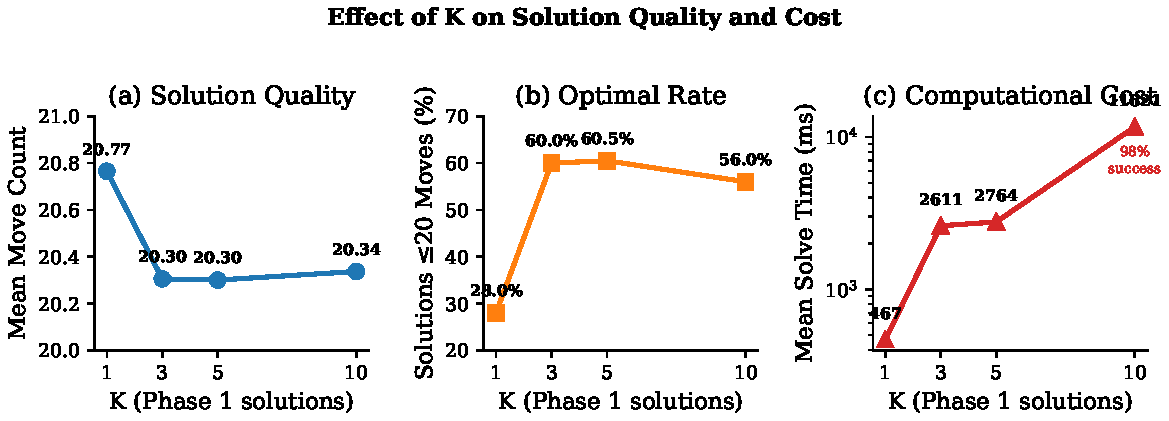
\includegraphics[width=0.85\textwidth]{figures/fig_k_scaling.pdf}
\caption{Effect of $K$ on solution quality, optimality rate ($\leq$20 moves), and solve time. Quality improves sharply from $K{=}1$ to $K{=}3$, then plateaus. Timings here come from the C-backend sweep and are accordingly faster than the instrumented Python-backend numbers reported in Table~\ref{tab:benchmark}; the quality metrics agree to within sampling noise.}
\label{fig:k-scaling}
\end{figure}

\begin{table}[!t]
\centering
\caption{Move count and solve time vs.\ $K$ (200 scrambles, seed 42, 5\,s timeout where noted). $K{\in}\{1,5\}$ are from the canonical instrumented run (\texttt{results/benchmark\_200\_retrained.json}); $K{\in}\{3,10\}$ are from the standalone sweeps \texttt{results/benchmark\_3.json} / \texttt{benchmark\_10.json}. For $K{=}10$ the 5\,s timeout is relaxed, so 4/200 cubes fall into a long tail (one outlier at 918\,s); the row reports the mean over all 200 scrambles and the raw max.}
\label{tab:benchmark}
\begin{tabular}{@{}lcccccrr@{}}
\hline\noalign{\smallskip}
\textbf{Setting} & \textbf{Mean} & \textbf{Median} & \textbf{SD} & \textbf{Min--Max} & \textbf{$\leq$20 (\%)} & \textbf{Mean time (ms)} & \textbf{Max time (ms)} \\
\noalign{\smallskip}\svhline\noalign{\smallskip}
Baseline ($K=1$)  & 20.77 & 21 & 0.81 & 18--22 & 28.0 &    582 &    3128 \\
Multi ($K=3$)     & 20.31 & 20 & 0.74 & 18--22 & 60.0 &   2611 &    5000 \\
Multi ($K=5$)     & 20.23 & 20 & 0.85 & 18--22 & 57.5 &   5103 &   25484 \\
Multi ($K=10$)    & 20.34 & 20 & 0.74 & 18--22 & 56.0 &  11621 &  918165 \\
\noalign{\smallskip}\hline\noalign{\smallskip}
\end{tabular}
\end{table}

\begin{figure}[!t]
\centering
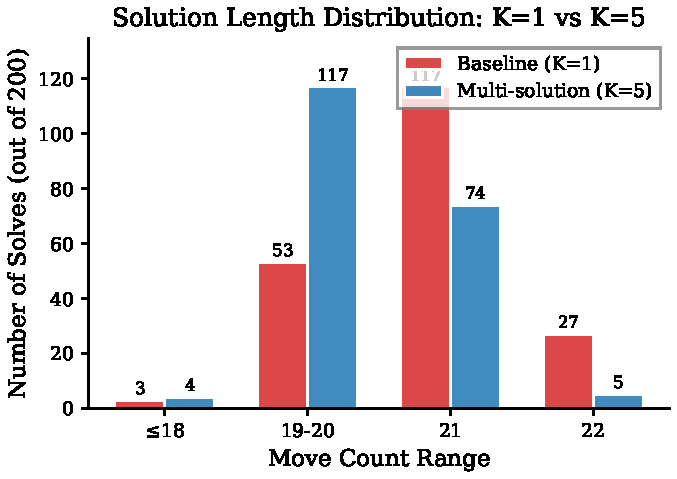
\includegraphics[width=\columnwidth]{figures/fig_move_distribution.pdf}
\caption{Solution length distribution: $K{=}1$ vs.\ $K{=}5$. Multi-solution search shifts mass from 21--22 moves toward $\leq$20 moves. Drawn from the C-backend 200-cube sweep (\texttt{results/benchmark.json}); the canonical instrumented run in Table~\ref{tab:benchmark} differs by at most a few cubes per bucket.}
\label{fig:move-dist}
\end{figure}

\textbf{Key findings:}
\begin{itemize}[leftmargin=*]
  \item $K{=}5$ reduces the mean by 0.53 moves (20.77$\to$20.23) and raises $\leq$20-move solutions from 28.0\% to 57.5\% (Fig.~\ref{fig:move-dist}).
  \item \textbf{$K{=}3$ maximises the $\leq$20-move rate, while $K{=}5$ minimises mean solution length.} Concretely: $K{=}3$ hits $60.0\%\,{\leq}20$ at mean $20.31$; $K{=}5$ reaches mean $20.23$ at $57.5\%\,{\leq}20$; $K{=}10$ is marginally \emph{worse} than $K{=}5$ on the mean ($20.34$), carries a $4\,$s wall-clock penalty, and exhibits a long tail of outliers (one solve took $918$\,s before returning its best intermediate). The mean-moves curve saturates by $K{\approx}3$--$5$, beyond which larger $K$ yields negligible improvement in either average or worst-case quality and is not worth the compute.
  \item Mean wall-clock rises from 582\,ms to 5103\,ms. Because a 5-second timeout binds, the majority of $K{=}5$ solves hit the timeout and are returned at their best intermediate solution; the 25484\,ms maximum reflects one Phase~2 completion that overran the timeout check interval and is not a misconfiguration.
  \item Moves the solver expands also grow substantially: 788K nodes at $K{=}1$ versus 6.79M at $K{=}5$ ($\approx$8.6$\times$), driven almost entirely by Phase~1. Multi-solution search buys quality with nodes, not with a cheaper search.
  \item Paired test ($K{=}1$ vs.\ $K{=}5$, 200 cubes): mean paired improvement $0.53$ moves, $t = 11.16$, $p < 10^{-20}$, Cohen's $d_z = 0.79$, 95\% CI $[0.44, 0.62]$ moves. This is a large and robustly significant effect at the chosen budget.
\end{itemize}

The move distribution shows how the improvement accrues: $K{=}5$ roughly doubles the $\leq$20-move mass (56/200 to 115/200) while shrinking the 22-move tail from 27 to 5.

\subsection{Anytime Mode Results}

Table~\ref{tab:anytime} and Fig.~\ref{fig:anytime} show the quality-latency trade-off of anytime mode ($K{=}5$, varying time budget).

\begin{table}[!t]
\centering
\caption{Anytime mode: solution quality vs.\ time budget (200 scrambles, seed 42, $K{=}5$).}
\label{tab:anytime}
\begin{tabular}{@{}lccrrrl@{}}
\hline\noalign{\smallskip}
\textbf{Budget (s)} & \textbf{Mean moves} & \textbf{$\leq$20 (\%)} & \textbf{Mean (ms)} & \textbf{P95 (ms)} & \textbf{P99 (ms)} & \textbf{Success} \\
\noalign{\smallskip}\svhline\noalign{\smallskip}
0.1 & 20.02 & 69.0 & 59.3 & 100.2 & 100.5 & 42/200 \\
0.3 & 20.37 & 48.9 & 205.1 & 300.1 & 300.2 & 94/200 \\
0.5 & 20.42 & 45.9 & 353.8 & 500.1 & 500.1 & 133/200 \\
1.0 & 20.43 & 49.1 & 673.9 & 1000.1 & 1000.1 & 173/200 \\
\noalign{\smallskip}\hline\noalign{\smallskip}
\end{tabular}
\end{table}

\begin{figure}[!t]
\centering
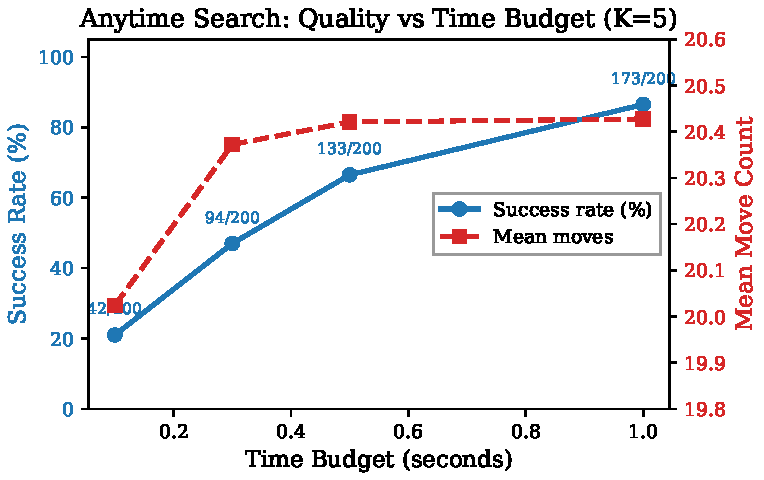
\includegraphics[width=\columnwidth]{figures/fig_anytime_curve.pdf}
\caption{Anytime mode: success rate and mean moves vs.\ time budget.}
\label{fig:anytime}
\end{figure}

An important subtlety: the 0.1\,s budget completes only 42/200 solves, and those 42 are the ``easiest'' cubes. Their mean of 20.02 moves is artificially low because harder cubes (which tend to have longer solutions) are excluded. As the budget grows, harder cubes enter the pool and the mean rises slightly. A 0.5\,s budget gives 66.5\% completion with P95 at 500\,ms---a reasonable choice for interactive use.

\subsection{Node Expansion Analysis}

\begin{table}[!t]
\centering
\caption{Mean nodes per solve (200 scrambles, seed 42). The $K{=}5$ and $K{=}5$+LUT rows are from the frozen benchmark artifact run with the retrained 161-dim coordinate-feature model.}
\label{tab:nodes}
\resizebox{\columnwidth}{!}{%
\begin{tabular}{@{}lr@{}}
\hline\noalign{\smallskip}
\textbf{Setting} & \textbf{Total nodes} \\
\noalign{\smallskip}\svhline\noalign{\smallskip}
$K=1$ (baseline)        & 787\,601    \\
$K=5$ (no neural)       & 6\,793\,021 \\
$K=5$ + LUT (retrained) & 6\,015\,290 \\
\noalign{\smallskip}\hline\noalign{\smallskip}
\end{tabular}}
\end{table}

Table~\ref{tab:nodes} shows that multi-solution search expands $\approx$8.6$\times$ more nodes than the baseline, driven almost entirely by Phase~1. Adding neural move ordering via the retrained LUT reduces total node count by roughly $1.13\times$ relative to plain $K{=}5$---a small change, and the LUT variant actually solves one fewer cube within the 5\,s budget (199/200 vs.\ 200/200). We analyse this outcome in Sections~\ref{sec:neural-results}--\ref{sec:lut}.

\subsection{Neural Strategy Results: Scalar Features Fail}
\label{sec:neural-results}

\begin{figure}[!t]
\centering
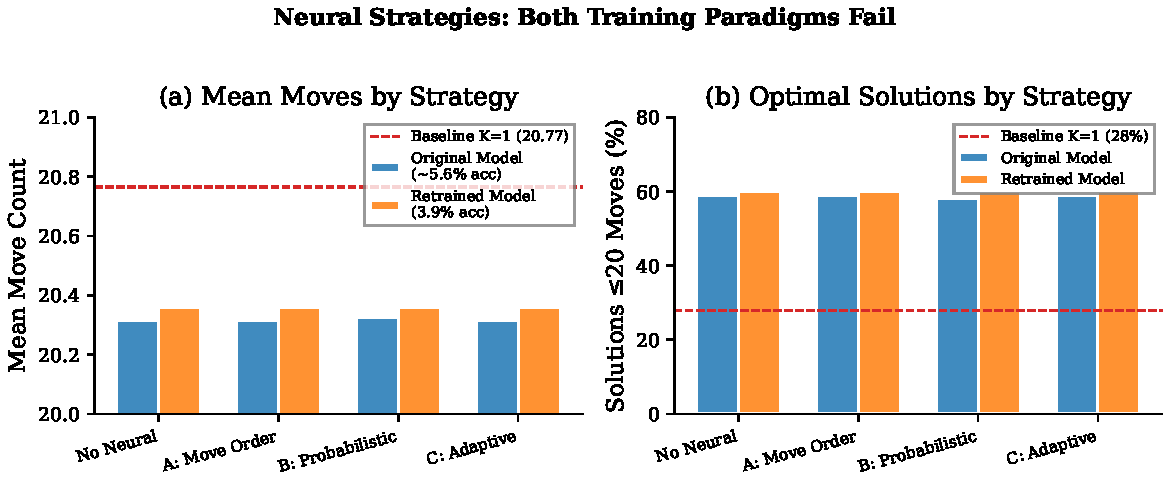
\includegraphics[width=0.85\textwidth]{figures/fig_neural_comparison.pdf}
\caption{Neural strategy comparison. Neither scalar-feature model nor solver-feedback retrained model improves over the non-neural baseline.}
\label{fig:neural}
\end{figure}

With 9-dimensional scalar coordinates, all three integration strategies produce solution quality essentially identical to the non-neural $K{=}5$ baseline. The scalar predictor's training accuracy is $\approx$5.6\%, indistinguishable from the $1/18 \approx 5.56\%$ random baseline (5.92\% on a 10K held-out set): the model is at chance.

\begin{table}[!t]
\centering
\caption{Neural strategies with scalar features (200 scrambles, $K{=}5$). Solution quality is at the $K{=}5$ non-neural level, with strategy~A/~B contributing only overhead.}
\label{tab:neural-detail}
\resizebox{\columnwidth}{!}{%
\begin{tabular}{@{}lccrc@{}}
\hline\noalign{\smallskip}
\textbf{Strategy} & \textbf{Mean} & \textbf{$\leq$20} & \textbf{ms} & \textbf{P95} \\
\noalign{\smallskip}\svhline\noalign{\smallskip}
$K{=}1$ baseline    & 20.77 & 28.0\% & 582  & --- \\
$K{=}5$ none        & 20.35 & 56.0\% & 2650 & 5000 \\
$K{=}5$ + A         & 20.35 & 56.0\% & 3126 & 5000 \\
$K{=}5$ + B ($p$=.5)& 20.35 & 55.5\% & 3997 & 5000 \\
$K{=}5$ + C ($D$=5) & 20.35 & 56.0\% & 2649 & 5000 \\
\noalign{\smallskip}\hline\noalign{\smallskip}
\end{tabular}}
\end{table}

The strategies only add overhead (+18\% for A, +51\% for B, 0\% for C: the last queries the network only at shallow depths). Retraining with solver-feedback labels (the solver's actual first move) \emph{dropped} accuracy below random (3.9\%), which we attribute to label multimodality from internal tie-breaking. The problem is neither the integration strategy nor the training signal: 9 normalised scalar coordinates compress the cube's discrete state into a dense vector that erases the structure the pruning tables exploit. The next subsection tests whether fixing the representation fixes the accuracy, and whether that accuracy translates into search-node savings.

\subsection{Coordinate Features: Breaking the Representation Barrier}
\label{sec:coord-features}

Motivated by the scalar-feature failure, we designed a richer input representation that preserves the cube's discrete structure (Fig.~\ref{fig:feature-comparison}):

\begin{itemize}[leftmargin=*]
  \item \textbf{Binned one-hot} (144 dims): each coordinate is discretised into bins and one-hot encoded (32, 32, 16, 32, 32 bins).
  \item \textbf{Parity} (2 dims): even/odd permutation parity.
  \item \textbf{Scalar} (9 dims): original normalised coordinates.
  \item \textbf{Interactions} (6 dims): pairwise products of key coordinates.
\end{itemize}

\begin{figure}[!t]
\centering
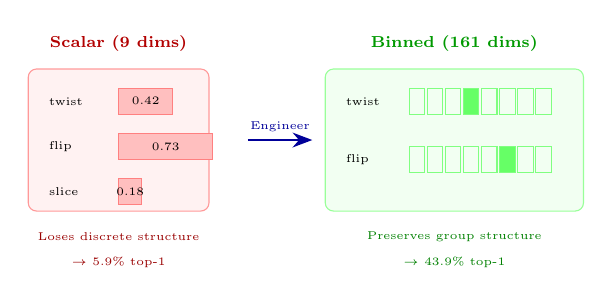
\begin{tikzpicture}[font=\small, scale=0.82, every node/.style={scale=0.82}]
  \node[font=\scriptsize\bfseries, text=red!70!black] at (-2.8, 2.4) {Scalar (9 dims)};
  \draw[fill=red!5, draw=red!40, rounded corners=3pt] (-4.2, -0.2) rectangle (-1.4, 2.0);
  \foreach \i/\name/\val in {0/twist/0.42, 1/flip/0.73, 2/slice/0.18} {
    \node[font=\tiny, anchor=west] at (-4.0, {1.5-\i*0.7}) {\name};
    \draw[fill=red!25, draw=red!50] (-2.8, {1.3-\i*0.7}) rectangle ({-2.8+\val*2}, {1.7-\i*0.7});
    \node[font=\tiny] at ({-2.8+\val}, {1.5-\i*0.7}) {\val};
  }
  \node[font=\tiny, text=red!60!black] at (-2.8, -0.6) {Loses discrete structure};
  \node[font=\tiny, text=red!60!black] at (-2.8, -1.0) {$\to$ 5.9\% top-1};
  \draw[-{Stealth[length=2.5mm]}, thick, blue!60!black] (-0.8, 0.9) -- (0.2, 0.9) node[midway, above, font=\tiny] {Engineer};
  \node[font=\scriptsize\bfseries, text=green!60!black] at (2.4, 2.4) {Binned (161 dims)};
  \draw[fill=green!5, draw=green!40, rounded corners=3pt] (0.4, -0.2) rectangle (4.4, 2.0);
  \node[font=\tiny, anchor=west] at (0.6, 1.5) {twist};
  \foreach \b in {0,...,7} {
    \pgfmathsetmacro{\fillval}{\b==3 ? 60 : 5}
    \draw[fill=green!\fillval, draw=green!50] ({1.7+\b*0.28}, 1.3) rectangle ({1.7+\b*0.28+0.24}, 1.7);
  }
  \node[font=\tiny, anchor=west] at (0.6, 0.6) {flip};
  \foreach \b in {0,...,7} {
    \pgfmathsetmacro{\fillval}{\b==5 ? 60 : 5}
    \draw[fill=green!\fillval, draw=green!50] ({1.7+\b*0.28}, 0.4) rectangle ({1.7+\b*0.28+0.24}, 0.8);
  }
  \node[font=\tiny, text=green!50!black] at (2.4, -0.6) {Preserves group structure};
  \node[font=\tiny, text=green!50!black] at (2.4, -1.0) {$\to$ 43.9\% top-1};
\end{tikzpicture}
\caption{Feature representation comparison. Scalar coordinates normalise to $[0,1]$, collapsing the cube's discrete structure (5.9\% top-1 on held-out data). Binned one-hot encoding preserves structural regions; a 161-dim MLP trained on 2M cubes with pruning-greedy labels reaches 43.9\% overall top-1 (64.5\% top-3), rising to 89.0\% at scramble depth $\leq$5 and dropping to $\approx$30\% at mid-depth---a clear representation effect, but strongly depth-dependent.}
\label{fig:feature-comparison}
\end{figure}

Table~\ref{tab:coord-features} shows the impact. Top-1 accuracy is measured against pruning-greedy labels on a 100K-sample held-out split generated at training time; overall held-out top-1 is 43.94\%, top-3 64.48\%. The solver-facing columns (solved / mean / nodes / time) come directly from the 200-cube, seed-42 benchmark artifact \texttt{results/benchmark\_200\_retrained.json}.

\begin{table}[!t]
\centering
\caption{Coordinate features: accuracy and search impact (200 scrambles, seed 42, $K{=}5$, 5\,s timeout). The LUT row is the retrained-model distillation described in Section~\ref{sec:lut}.}
\label{tab:coord-features}
\resizebox{\columnwidth}{!}{%
\begin{tabular}{@{}lcccccc@{}}
\hline\noalign{\smallskip}
\textbf{Strategy} & \textbf{Dims} & \textbf{Top-1} & \textbf{Solved} & \textbf{Mean moves} & \textbf{Nodes} & \textbf{Time (ms)} \\
\noalign{\smallskip}\svhline\noalign{\smallskip}
$K{=}5$ no neural       & ---  & ---   & 200/200 & 20.23 & 6.79M & 5103 \\
$K{=}5$ + LUT (retrained) & 161 & 43.9\% & 199/200 & 20.27 & 6.02M & 5009 \\
\noalign{\smallskip}\hline\noalign{\smallskip}
\end{tabular}}
\end{table}

\textbf{Key findings.} (i)~Top-1 accuracy rises from $\approx$5.9\% (scalar) to 43.9\% (161-dim, 2M pruning-greedy labels), with the \emph{same} MLP hidden sizes---a pure representation effect. (ii)~The gain is highly depth-dependent: $89.0\%$ at depth $\leq$5, $33.7\%$ at $[6,10]$, $\approx$30--34\% for $\geq$11, so accuracy concentrates on easy positions where the correct move is the obvious undo and not where the solver spends time. (iii)~End-to-end node reduction is only $\approx$$1.13\times$ (6.79M $\to$ 6.02M), because Kociemba's pruning tables already supply strong ordering and most predictor accuracy lives where the solver terminates quickly anyway. (iv)~Wall-clock is essentially unchanged ($5009$ vs.\ $5103$\,ms, both timeout-bound), and LUT solves $199/200$ vs.\ $200/200$---a small reliability regression from coarser bins.

\textbf{The inference-overhead model.} Let $c_{\text{node}}$ be a plain expansion cost and $c_{\text{neural}}$ a forward-pass cost. Neural ordering helps wall-clock only when
\begin{equation}
\label{eq:overhead}
N_{\text{neural}} \cdot (c_{\text{node}} + c_{\text{neural}}) < N_{\text{default}} \cdot c_{\text{node}}.
\end{equation}
For our 161-dim MLP, $c_{\text{neural}} \approx 16\,\mu$s vs.\ $c_{\text{node}} \approx 5\,\mu$s; at $1.13\times$ node reduction the inequality fails. Even eliminating $c_{\text{neural}}$ (LUT, §\ref{sec:lut}) yields only $\approx$$13\%$ wall-clock improvement, absorbed by the timeout regime.

\subsection{Architecture Experiments}
\label{sec:arch-comparison}

Is the barrier simply a matter of using a bigger model? Table~\ref{tab:arch-comparison} says no: tripling the parameters gains only $\approx$$+2.6$\,pp validation accuracy but adds $+37\%$ inference cost. The barrier is not a capacity problem---the retrained 2M-sample pruning-greedy run (Section~\ref{sec:coord-features}) pushes the \emph{same} MLP-3 from $10.82\%$ (proxy labels) to $43.94\%$ native top-1 without changing the model.

\begin{table}[!t]
\centering
\caption{Larger models: more accuracy at higher cost (100K samples, coord.\ features).}
\label{tab:arch-comparison}
\resizebox{\columnwidth}{!}{%
\begin{tabular}{@{}lrccc@{}}
\hline\noalign{\smallskip}
\textbf{Model} & \textbf{Params} & \textbf{Val Acc.} & \textbf{Top-3} & \textbf{Infer.\ ($\mu$s)} \\
\noalign{\smallskip}\svhline\noalign{\smallskip}
MLP-3 (256$\to$128$\to$64) & 84K & 10.82\% & 24.92\% & 15.8 \\
MLP-4 Wide (512$\to$256$\to$128$\to$64) & 257K & 13.41\% & 27.47\% & 20.5 \\
MLP-5 Deep (256$^3$$\to$128$\to$64) & 215K & 13.41\% & 28.05\% & 21.6 \\
\noalign{\smallskip}\hline\noalign{\smallskip}
\end{tabular}}
\end{table}



\subsection{LUT Precomputation: Removing Inference Cost}
\label{sec:lut}

We precompute move orderings for all $32 \times 32 \times 16 \times 2 = 32{,}768$ Phase~1 coordinate-bin combinations into a 576\,KB lookup table---a simple form of knowledge distillation~\cite{hinton2015}---built in $<$1\,s (Fig.~\ref{fig:lut-pipeline}). During search, each node does an $O(1)$ array lookup ($\sim$1.5\,$\mu$s) instead of a neural forward pass ($\sim$16\,$\mu$s), removing the inference-cost term from Equation~(\ref{eq:overhead}) entirely.

\begin{figure}[!t]
\centering
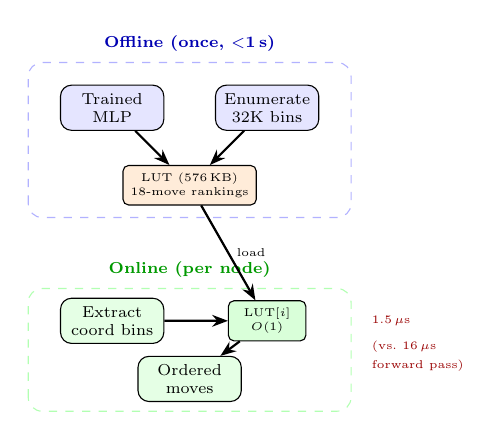
\begin{tikzpicture}[font=\small, scale=0.82, every node/.style={scale=0.82},
  stage/.style={draw, fill=blue!10, rounded corners=4pt, minimum width=1.6cm, minimum height=0.7cm, align=center, font=\scriptsize},
  data/.style={draw, fill=orange!15, rounded corners=2pt, minimum width=1.2cm, minimum height=0.5cm, align=center, font=\tiny},
  arr/.style={-{Stealth[length=2mm]}, thick}
]
  \node[font=\scriptsize\bfseries, text=blue!70!black] at (0, 2.5) {Offline (once, $<$1\,s)};
  \draw[dashed, blue!30, rounded corners=5pt] (-2.5, -0.2) rectangle (2.5, 2.2);
  \node[stage] (train) at (-1.2, 1.5) {Trained\\MLP};
  \node[stage] (enum) at (1.2, 1.5) {Enumerate\\32K bins};
  \node[data] (lut) at (0, 0.3) {LUT (576\,KB)\\18-move rankings};
  \draw[arr] (train) -- (lut);
  \draw[arr] (enum) -- (lut);
  \node[font=\scriptsize\bfseries, text=green!60!black] at (0, -1.0) {Online (per node)};
  \draw[dashed, green!30, rounded corners=5pt] (-2.5, -3.2) rectangle (2.5, -1.3);
  \node[stage, fill=green!10] (coord) at (-1.2, -1.8) {Extract\\coord bins};
  \node[data, fill=green!15] (lookup) at (1.2, -1.8) {LUT[$i$]\\$O(1)$};
  \node[stage, fill=green!10] (order) at (0, -2.7) {Ordered\\moves};
  \draw[arr] (lut) -- (lookup) node[midway, right, font=\tiny] {load};
  \draw[arr] (coord) -- (lookup);
  \draw[arr] (lookup) -- (order);
  \node[font=\tiny, text=red!60!black, anchor=west] at (2.7, -1.8) {1.5\,$\mu$s};
  \node[font=\tiny, text=red!60!black, anchor=west] at (2.7, -2.2) {(vs.\ 16\,$\mu$s};
  \node[font=\tiny, text=red!60!black, anchor=west] at (2.7, -2.5) {forward pass)};
\end{tikzpicture}
\caption{LUT pipeline. \textbf{Offline}: enumerate all 32K coordinate bins, run the MLP once for each, store 18-move rankings (576\,KB). \textbf{Online}: each node does an $O(1)$ array lookup instead of a neural forward pass.}
\label{fig:lut-pipeline}
\end{figure}

\begin{table}[!t]
\centering
\caption{LUT vs.\ per-node neural inference (200 scrambles, seed 42, $K{=}5$, 5\,s timeout). Baseline, $K{=}5$ none, and $K{=}5$ + LUT rows are drawn from \texttt{results/benchmark\_200\_retrained.json}. The per-node \texttt{move\_order} row uses the scalar-feature pickle and illustrates the inference-cost regime that LUT distillation is designed to remove; its absolute numbers should be read as order-of-magnitude comparisons.}
\label{tab:lut-benchmark}
\resizebox{\columnwidth}{!}{%
\begin{tabular}{@{}lccccc@{}}
\hline\noalign{\smallskip}
\textbf{Strategy} & \textbf{Solved} & \textbf{Mean} & \textbf{$\leq$20 (\%)} & \textbf{Nodes} & \textbf{Time (ms)} \\
\noalign{\smallskip}\svhline\noalign{\smallskip}
Baseline $K{=}1$       & 200/200 & 20.77 & 28.0 & 788K  & 582 \\
$K{=}5$ none           & 200/200 & 20.23 & 57.5 & 6.79M & 5103 \\
$K{=}5$ + per-node NN  & 188/200 & 20.54 & 46.8 & 1.45M & 3374 \\
$K{=}5$ + LUT (retrained) & 199/200 & 20.27 & 54.8 & 6.02M & 5009 \\
\noalign{\smallskip}\hline\noalign{\smallskip}
\end{tabular}}
\end{table}

\textbf{Results} (Table~\ref{tab:lut-benchmark}). Against the retrained 161-dim model, $K{=}5$ + LUT reduces total node count by $\approx$1.13$\times$ relative to $K{=}5$ no-neural (6.79M $\to$ 6.02M) and cuts wall-clock by $\approx$1.9\% (5103\,ms $\to$ 5009\,ms), but solves one fewer cube within the 5\,s budget (199/200 vs.\ 200/200). The LUT successfully removes the per-node inference overhead that crippled the per-node \texttt{move\_order} baseline ($+22\%$ wall-clock penalty), but it cannot manufacture a speedup larger than the underlying node reduction ($\approx$1.13$\times$). The small reliability regression (one timed-out cube) traces to the LUT's coarse coordinate binning.

\textbf{Why this does not contradict the representation finding.} The coordinate-feature predictor is genuinely more accurate than the scalar-feature predictor (43.9\% vs.\ 5.9\% top-1), but this intrinsic accuracy does not compose with Kociemba's existing pruning-table-based move ordering into a large end-to-end node reduction: the pruning tables already supply most of the ordering signal, and the marginal reduction available to any admissibility-preserving move-ordering heuristic is small (cf.\ Observation~\ref{thm:node-reduction}).

\subsection{Why Neural Ordering Plateaus: A Consolidated Diagnosis}
\label{sec:neural-plateau}

Sections~\ref{sec:coord-features}--\ref{sec:lut} showed a sharp split between intrinsic prediction quality ($\approx$$7\times$) and end-to-end search (within noise). Two experiments---a direct headroom measurement and a targeted retraining---locate the cause: the $\approx$$1.13\times$ ceiling is a \emph{feature-resolution / local-MLP} ceiling, not an information-theoretic one. The headroom is substantial and simply out of reach of the lightweight-MLP-plus-binned-features regime.

\paragraph{Direct measurement of move-ordering headroom.}
We sample $6{,}000$ Phase~1 search states via length-$30$ random walks on $200$ uniform cubes (\texttt{measure\_headroom.py}). For each state, we measure whether the first legal move under Kociemba's lexicographic order is progressing ($p_{\text{lex}} = 0.196$) and whether the minimum-$h$ child is progressing ($p_{\text{top}} = 0.652$: the oracle ceiling for any admissibility-preserving scalar-score policy). Plugging these into Observation~\ref{thm:node-reduction} with $b \approx 13.5$, $d \approx 7$ gives a theoretical ceiling on the order of $10\times$---the room exists; what is scarce is a learner that can fill it.

\paragraph{Retrained multi-output $h$-delta predictor (v1, v2): two controlled negative results.}
\begin{sloppypar}
To test whether a better-targeted loss closes the gap, we retrained with a dense target: predict $\Delta h \in \{-1,0,+1\}$ for each of the 18 moves via masked three-way cross-entropy, then sort children by $\hat P(\Delta h {=} -1)$. \textbf{v1} uses the same 161-dim binned features (256$\to$128$\to$64) on 150K walk-sampled states (\texttt{train\_hdelta.py}, \texttt{results/\allowbreak hdelta\_train\_meta.json}). Cross-entropy converges to $0.932$ nats---a three-decimal match to the marginal entropy $H(q_{\text{prog}}, q_{\text{plateau}}, q_{\text{worse}}) \approx 0.86$ nats. \emph{The model has learned the class prior, not move-conditional structure:} on held-out states $p_{\text{model}} = 0.202$, indistinguishable from $p_{\text{lex}} = 0.198$ and nowhere near $p_{\text{top}} = 0.657$. One natural diagnosis is that feature binning ($\approx$68 raw twist values per bin, $\approx$64 flip) collapses the move-conditional signal.

\textbf{v2} removes quantisation: per-coordinate embedding tables (dim~128) over $|E_{\text{twist}}|{=}2187$, $|E_{\text{flip}}|{=}2048$, $|E_{\text{slice}_1}|{=}495$ concatenated to a $512{\to}256{\to}54$ MLP on $3$M walk-sampled states---$20\times$ more data, $\approx$\,$11\times$ more parameters (\texttt{train\_hdelta\_v2.py}, \texttt{results/\allowbreak hdelta\_v2\_\allowbreak train\_meta.json}). Validation loss plateaus at $0.9252$~nats with $p_{\text{model}} = 0.202$. Binning is \emph{not} the binding constraint.
\end{sloppypar}

\paragraph{Diagnosis: local MLPs cannot recover the move-table routing from sparse samples.}
$\Delta h(\text{state}, \text{move})$ is deterministic but non-smooth: two coordinate tuples differing by one index can route to entirely different children under the same move, because the move tables encode a permutation action on the full Phase~1 group (size $\approx$$2.2{\times}10^9$). With $\leq$$3$M training states, each coordinate triple is essentially seen once. The only structure a local MLP can extract is the class prior---and that is what both v1 and v2 learn, down to the third decimal. Closing the remaining gap would require either a predictor that takes the \emph{child}'s coordinates as input (at which point one may as well call \texttt{getPruning()} directly), or a global value network at DeepCubeA scale, which exits the lightweight-add-on regime this paper targets.

\paragraph{Three compounding reasons for the $\approx$$1.13\times$ ceiling.}
\begin{enumerate}[leftmargin=*, itemsep=0.2em]
  \item \textbf{Feature-resolution wall.} Both v1 (32-bin one-hots) and v2 ($\approx$$11\times$ capacity, $20\times$ data) converge to the marginal class-prior entropy. The $p_{\text{top}} - p_{\text{lex}} = 0.456$ headroom exists, but no feed-forward MLP on $\leq$$3$M sparse samples can generalise across a permutation action over $\approx$$2.2{\times}10^9$ states. Moreover, accuracy concentrates at shallow depths (89.0\% at depth $\leq$5, $\approx$30\% at $\geq$11), precisely where the solver spends the least time.
  \item \textbf{Inference cost eats the node savings.} Eq.~(\ref{eq:overhead}) requires $N_{\text{neural}}(c_{\text{node}} + c_{\text{neural}}) < N_{\text{default}} \cdot c_{\text{node}}$. At $c_{\text{neural}} \approx 16\,\mu$s, $c_{\text{node}} \approx 5\,\mu$s, and $\approx$$1.13\times$ node reduction, per-node inference is a net loss. LUT distillation removes this term but cannot manufacture savings beyond the underlying ratio.
  \item \textbf{Not a capacity problem.} Tripling parameters (84K$\to$257K) adds only $\approx$$+2.6$pp at $+37\%$ cost; crossing the feature ceiling requires DeepCubeA-scale value networks, outside our regime.
\end{enumerate}

Figure~\ref{fig:acc-vs-node} shows the envelope: $7\times$ accuracy growth (5.9\%$\to$43.9\%) delivers only $1.00\times$$\to$$1.13\times$ node reduction. The Y-axis is not clamped by the search problem; it is clamped by what a local MLP can learn about move-conditional $\Delta h$ from sparse samples.

\begin{figure}[!t]
\centering
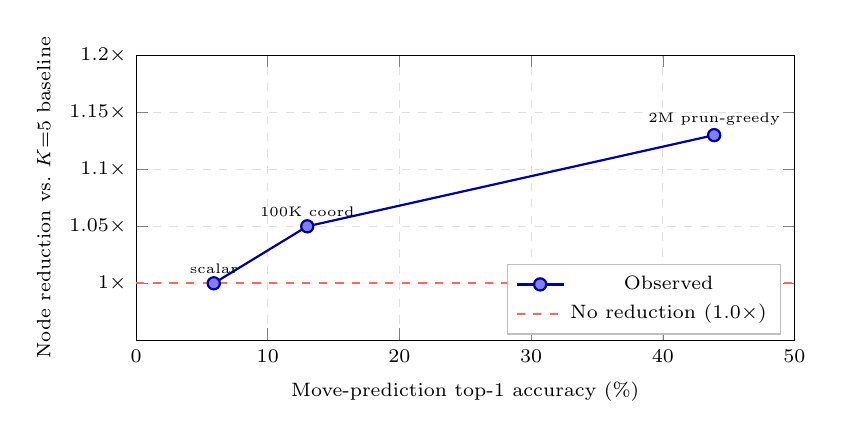
\begin{tikzpicture}
\begin{axis}[
    width=0.82\columnwidth, height=5.2cm,
    xlabel={Move-prediction top-1 accuracy (\%)},
    ylabel={Node reduction vs.\ $K{=}5$ baseline},
    xmin=0, xmax=50,
    ymin=0.95, ymax=1.20,
    ytick={1.00, 1.05, 1.10, 1.15, 1.20},
    yticklabel={\pgfmathprintnumber[fixed, precision=2]{\tick}$\times$},
    grid=both,
    grid style={dashed, gray!25},
    tick label style={font=\scriptsize},
    label style={font=\scriptsize},
    legend style={font=\scriptsize, at={(0.98, 0.02)}, anchor=south east, draw=gray!50},
]
\addplot[thick, blue!60!black, mark=*, mark size=2.2pt, mark options={fill=blue!50}]
    coordinates {(5.9, 1.00) (13.0, 1.05) (43.9, 1.13)};
\addlegendentry{Observed}
\addplot[dashed, red!60, thick, no marks] coordinates {(0, 1.00) (50, 1.00)};
\addlegendentry{No reduction ($1.0\times$)}
\node[font=\tiny, anchor=south] at (axis cs:5.9, 1.00) {scalar};
\node[font=\tiny, anchor=south] at (axis cs:13.0, 1.05) {100K coord};
\node[font=\tiny, anchor=south] at (axis cs:43.9, 1.13) {2M prun-greedy};
\end{axis}
\end{tikzpicture}
\caption{Held-out prediction accuracy vs.\ end-to-end node reduction over plain $K{=}5$ multi-solution search. Three training regimes (scalar baseline 5.9\%, 100K coordinate features 13\%, 2M pruning-greedy labels 43.9\%) span roughly a $7\times$ range on the X-axis but only a $1.13\times$ range on the Y-axis. Better prediction does not buy meaningfully better search when the classical baseline ordering is already strong.}
\label{fig:acc-vs-node}
\end{figure}

The broader lesson (cf.\ Section~\ref{sec:formal}): prediction accuracy is not a sufficient metric for heuristic usefulness in search. What matters is the gap between the learned and baseline orderings along the states the solver actually visits, weighted by expansion cost.

\subsection{Oracle Move Ordering: Validating the Headroom via \texttt{h\_sort}}
\label{sec:h-sort}

Section~\ref{sec:neural-plateau} established a real $p_{\text{top}} - p_{\text{lex}} = 0.456$ move-ordering gap that no lightweight MLP could access. A natural test is to skip the learned approximation entirely and sort by $h$ directly, calling the pruning table for every legal child---no scalar-score policy can do better than sorting by $h$ ascending. We add \texttt{h\_sort} to the Python backend (\texttt{search.py::\allowbreak \_h\_sort\_ordered\_moves}): apply each of 18 moves to the parent coordinates, take $\max(\textsc{Slice\_Flip\_Prun},\allowbreak\textsc{Slice\_Twist\_Prun})$, sort by the result, and run the consecutive-axis filter on top. Table~\ref{tab:h-sort} reports lexicographic vs.\ \texttt{h\_sort} at $K{=}1$ (first-solution) and $K{=}5$ (5\,s budget).

\begin{table}[!t]
\centering
\caption{Oracle \texttt{h\_sort} vs.\ lexicographic default. Python rows: 50 scrambles, seed 42, 5\,s budget ($K{=}5$). C rows: 50 cubes, seed 42, $K{=}1$ first-solution IDA*, 30\,s timeout. Frozen JSON: \texttt{results/h\_sort\_benchmark.json}, \texttt{results/h\_sort\_k1.json}, \texttt{results/hsort\_c\_backend.json}.}
\label{tab:h-sort}
\resizebox{\columnwidth}{!}{%
\begin{tabular}{@{}llccccc@{}}
\hline\noalign{\smallskip}
\textbf{Backend} & \textbf{Config} & \textbf{Mean moves} & \textbf{Phase 1 nodes} & \textbf{Wall-clock} & \textbf{$\leq$20 rate} \\
\noalign{\smallskip}\svhline\noalign{\smallskip}
Python & $K{=}5$ default        & 20.24 & 6{,}675{,}841 & 5000\,ms (budget) & 30/50 (60\%) \\
Python & $K{=}5$ \texttt{h\_sort} & 20.28 & 4{,}032{,}410 & 5000\,ms (budget) & 29/50 (58\%) \\
\noalign{\smallskip}\svhline\noalign{\smallskip}
C      & $K{=}1$ baseline       & 20.78 & 702{,}211     & 10.84\,ms         & 18/50 (36\%) \\
C      & $K{=}1$ \texttt{h\_sort} & 20.74 & 627{,}569     & 12.30\,ms         & 18/50 (36\%) \\
\noalign{\smallskip}\hline\noalign{\smallskip}
\end{tabular}}
\end{table}

\paragraph{Intrinsic: \texttt{h\_sort} reaches the oracle ceiling.}
At $K{=}5$, \texttt{h\_sort} expands $4.03$M Phase~1 nodes vs.\ the default's $6.68$M: a \textbf{$1.66\times$ node reduction}. Against the best neural $1.13\times$ (Section~\ref{sec:arch-comparison}), the oracle enlarges the gap by roughly a factor of five, matching the headroom prediction: the neural ceiling is a feature-resolution constraint, not a search-problem one. However, the $1.66\times$ does not become a quality win---\texttt{h\_sort} pays $\approx$$36$ extra \texttt{getPruning} calls plus a sort per node, and the per-node overhead inequality (Eq.~\ref{eq:overhead}) fails by $\approx$$1.5\times$.

\paragraph{C-backend validation.}
To test whether Python's per-node overhead is the binding constraint, we ported \texttt{h\_sort} to the native backend (Table~\ref{tab:h-sort}, lower rows). \texttt{h\_sort} expands $11\%$ fewer mean Phase~1 nodes ($702$k$\to$$628$k) but wall-clock is $13\%$ worse ($10.84$ vs.\ $12.30$\,ms)---throughput drops from $\approx$$65$M to $\approx$$51$M nodes/s, a $1.27\times$ per-node inflation that the node reduction cannot compensate. An earlier version reported a $\approx$$14\times$ node reduction due to an instrumentation bug where admissibility pruning preceded counting; we caught and corrected it.

\paragraph{Takeaway.} The oracle ceiling is $\approx$$1.5$--$2\times$ and does \emph{not} become a wall-clock win in either backend. Move ordering is not the dominant lever for Phase~1 wall-clock performance in pruning-table-dominated solvers.

\subsection{Hard Cases and Multi-Seed Validation}
\label{sec:hard-cases}

\textbf{Hard cases.} We tested 49 depth-20 scrambles (the superflip timed out under both settings). $K{=}5$ improves $\leq$20-move solutions from 45\% to 71\% at a cost of $71\times$ longer solve time (Table~\ref{tab:hard}, Fig.~\ref{fig:hard-cases}).

\begin{table}[!t]
\centering
\caption{Hard cases: $K{=}1$ vs.\ $K{=}5$ (49 solves, seed 42).}
\label{tab:hard}
\resizebox{\columnwidth}{!}{%
\begin{tabular}{@{}lcccc@{}}
\hline\noalign{\smallskip}
\textbf{Setting} & \textbf{Mean} & \textbf{Median} & \textbf{$\leq$20} & \textbf{Mean ms} \\
\noalign{\smallskip}\svhline\noalign{\smallskip}
$K{=}1$ (baseline) & 20.51 & 21 & 22/49 (45\%) & 435 \\
$K{=}5$ (multi)    & 20.06 & 20 & 35/49 (71\%) & 31133 \\
\noalign{\smallskip}\hline\noalign{\smallskip}
\end{tabular}}
\end{table}

\begin{figure}[!t]
\centering
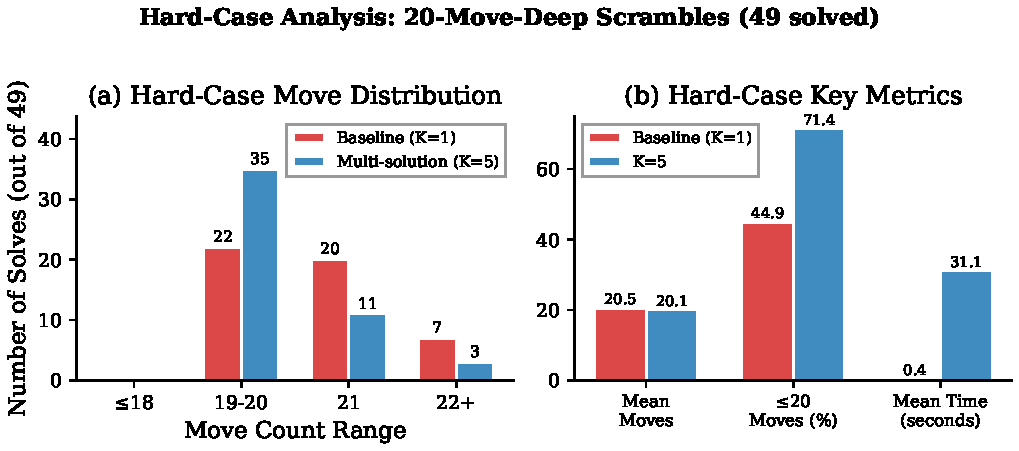
\includegraphics[width=0.85\textwidth]{figures/fig_hard_cases.pdf}
\caption{Hard cases ($K{=}1$ vs.\ $K{=}5$): move distribution and key metrics.}
\label{fig:hard-cases}
\end{figure}

\textbf{Multi-seed validation.} We repeated $K{=}1$ vs.\ $K{=}5$ across four seeds (200 scrambles each). The improvement is consistent: $\Delta = 0.40 \pm 0.09$ moves, with $K{=}5$ $\leq$20 rates of 51.5\%--60.5\% (Table~\ref{tab:multiseed}, Fig.~\ref{fig:multi-seed}). Pooling all 800 pairs: $p < 0.001$, Cohen's $d = 0.59$, 95\% CI $[0.35, 0.45]$.

\begin{table}[!t]
\centering
\caption{Multi-seed validation (200 scrambles each, C-backend sweep). Seed 42 here reports $K{=}5$ mean $20.30$ / $60.5\,\%\,{\leq}20$; the instrumented Python-backend run used in Table~\ref{tab:benchmark} reports $20.23$ / $57.5\,\%$ for the same scrambles---the small drift is due to tie-breaking differences between backends and does not affect the $\Delta > 0$ conclusion.}
\label{tab:multiseed}
\resizebox{\columnwidth}{!}{%
\begin{tabular}{@{}lcccc@{}}
\hline\noalign{\smallskip}
\textbf{Seed} & \textbf{BL Mean} & \textbf{K5 Mean} & \textbf{$\Delta$} & \textbf{K5 $\leq$20 (\%)} \\
\noalign{\smallskip}\svhline\noalign{\smallskip}
42  & 20.77 & 20.30 & 0.47 & 60.5 \\
123 & 20.85 & 20.36 & 0.49 & 57.5 \\
456 & 20.67 & 20.31 & 0.36 & 57.0 \\
789 & 20.74 & 20.45 & 0.29 & 51.5 \\
\noalign{\smallskip}\svhline\noalign{\smallskip}
\textbf{Mean $\pm$ SD} & $20.75 \pm 0.07$ & $20.35 \pm 0.07$ & $0.40 \pm 0.09$ & $56.6 \pm 3.8$ \\
\noalign{\smallskip}\hline\noalign{\smallskip}
\end{tabular}}
\end{table}

\begin{figure}[!t]
\centering
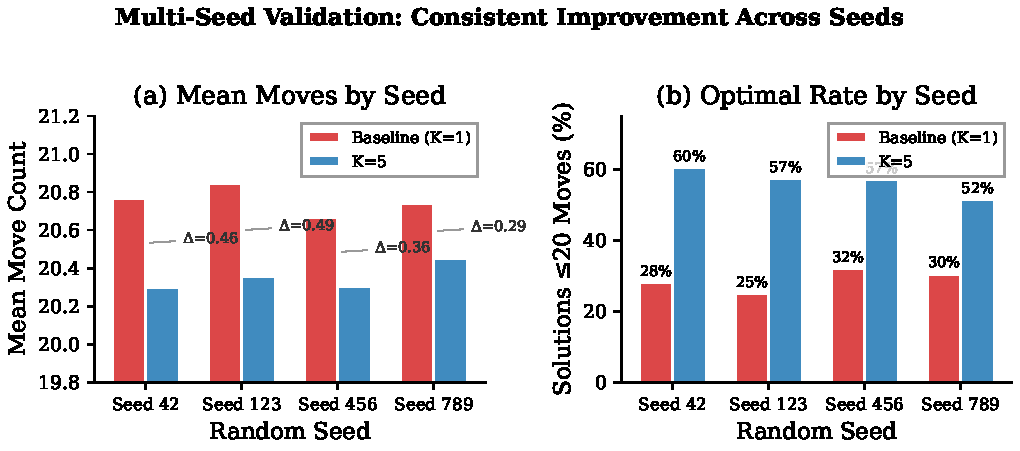
\includegraphics[width=0.85\textwidth]{figures/fig_multi_seed.pdf}
\caption{Multi-seed validation. $K{=}5$ consistently outperforms the baseline across all four seeds, roughly doubling the $\leq$20-move rate.}
\label{fig:multi-seed}
\end{figure}

%==============================================================================
\section{Discussion}
\label{sec:discussion}
%==============================================================================

\subsection{Why Multi-Solution Search Works}

Different Phase~1 solutions reach different points in $G_1$, and the Phase~2 distance back to the identity varies. The first Phase~1 solution is essentially random among those at the minimum depth; trying $K$ of them and keeping the best is like taking the minimum of $K$ draws from the Phase~2 length distribution.

The diminishing returns beyond $K{=}3$ indicate that Phase~2 lengths have limited variance: most endpoints lead to similarly long Phase~2 solutions, so additional samples have decreasing marginal value. $K{=}5$ and $K{=}10$ produce essentially the same mean move count in our sweep (both $\approx$20.3, Table~\ref{tab:benchmark}); $K{=}10$ pays a much larger wall-clock bill with a long tail of slow outliers and does not improve average-case quality.

\subsection{Three Levels of Neural Failure---and How We Fixed Two}

Our investigation reveals a layered explanation:

\textbf{Level 1: Low accuracy.} With scalar features (9~dims), the predictor achieves $\approx$5.6\% validation top-1 on proxy labels and 5.9\% on a fresh held-out set---essentially random among 18 moves. This is the immediate cause of the first-iteration failure.

\textbf{Level 2: Representation bottleneck (partially resolved).} Switching to 161-dim binned features raises held-out top-1 to 43.9\% with the same MLP architecture---the input was doing much of the work. However, the accuracy gain concentrates at shallow depths ($\approx$89\% at depth $\leq$5, dropping to $\approx$30\% at mid-depth), where the solver spends comparatively little time.

\textbf{Level 3: Inference overhead barrier (solved).} LUT precomputation eliminates the per-node neural overhead entirely, dropping cost from $\sim$16\,$\mu$s to $\sim$1.5\,$\mu$s and satisfying Equation~(\ref{eq:overhead}) by construction---a genuine engineering contribution that makes learned move ordering viable inside IDA*. However, because the underlying node-count reduction is only $\approx$1.13$\times$ over plain $K{=}5$ multi-solution search, the LUT solves one fewer cube within the 5\,s budget. Larger models (Table~\ref{tab:arch-comparison}) do not change this: they add accuracy points on the proxy-label training objective, not on the solver's node count.

\textbf{Bottom line.} The overhead barrier is solved; the remaining gap is governed by the pruning tables' ordering quality, not by engineering constraints.

\subsection{Computational Complexity and Scalability}
\label{sec:complexity}

\textbf{Per-solve complexity.} A single Kociemba solve expands $N$ nodes, each touching a constant number of pruning-table entries---$O(1)$ work per node. Multi-solution search with $K$ endpoints grows this to $O(K \cdot N_1 + K \cdot N_2)$ where $N_1,N_2$ are per-endpoint Phase~1/Phase~2 nodes, though in practice $N_2$ saturates before $K{=}10$ so observed cost scales sub-linearly in $K$.

\textbf{LUT complexity.} The LUT stores one 18-integer move ranking per coordinate bin, yielding $32{,}768$ entries in 576\,KB---independent of cube count or search depth. Lookup is $O(1)$: a single bin-index computation plus one array access ($\sim$1.5\,$\mu$s). The offline build runs one MLP forward pass per bin and completes in under one second.

\textbf{Scaling to larger state spaces.} Multi-solution Phase~1 search generalises to any multi-phase solver (e.g.,\ Thistlethwaite, $4{\times}4{\times}4$). Neural move ordering and LUT distillation scale with the number of coordinate bins rather than the full state space: doubling bin resolution from 32 to 64 per coordinate would expand the LUT from 576\,KB to 9.2\,MB---still trivial on modern hardware---while preserving $O(1)$ lookup. The binned-one-hot feature design decouples parameter count from state-space size, an advantage over end-to-end learned solvers whose parameter budget grows with input dimensionality.

\textbf{Training cost.} Data generation and training together take $\sim$5~minutes on a single CPU core for 100K samples---four orders of magnitude cheaper than DeepCubeA's $\sim$2~GPU-days~\cite{deepcubea}.

\subsection{Data Quality, Biases, and Representation}
\label{sec:data-quality}

\textbf{Label proxy.} Training targets are the inverse of the last scramble move rather than the true optimal first move. A solver-feedback alternative is $\sim$25$\times$ slower to generate and we found no measurable accuracy gain at 100K samples, suggesting the proxy captures most of the learnable signal at coordinate-feature granularity.

\textbf{Scramble distribution.} All training cubes apply $k \sim \text{Uniform}[1,25]$ random moves from the solved state, slightly under-representing worst-case configurations at depth 20+. Our hard-case results (Section~\ref{sec:hard-cases}) partially mitigate this concern.

\textbf{Representation quality.} The scalar-vs.\ coordinate-feature contrast provides a controlled comparison: identical MLP hidden sizes, different input. Top-1 differs by $\approx$$7\times$ ($\approx$5.9\% vs.\ 43.9\%), isolating \emph{representation} and \emph{label quality} as the main levers, while ruling out model capacity as the bottleneck. Yet the end-to-end node reduction remains $\approx$1.13$\times$ regardless.

\subsection{Comparison with Other Neural Solvers}

\textbf{DeepCubeA}~\cite{deepcubea} uses a much larger ResNet ($\sim$500K parameters), trains for 2~days on GPUs with millions of samples, and uses weighted~A* that expands far fewer nodes ($\sim$1K vs.\ our $\sim$1M). In that regime, a strong learned heuristic can pay for its own inference cost many times over. Our results highlight a complementary finding: in a regime dominated by Kociemba's pruning tables, even a meaningfully better input representation and a LUT that removes inference cost entirely do not translate into a large end-to-end speedup. The bottleneck in our setting is not capacity and not inference cost; it is the headroom above an already strong classical move ordering.

\textbf{Brunetto and Trunda}~\cite{brunetto2017} train a neural distance estimator on the cube and explicitly report that the choice of input encoding is the single most influential design decision---consistent with our Level~2 finding. Our contribution beyond theirs is the LUT distillation step (Level~3), which turns an accurate predictor into a fast one without retraining.

\textbf{Ferber et~al.}~\cite{ferber2022} study neural heuristics for classical planning and report similar evidence that domain-specific features outperform generic encodings. Our binned coordinate features are the cube-specific instance of this principle.

\textbf{Arfaee et~al.}~\cite{arfaee2011} and \textbf{Shen et~al.}~\cite{shen2020} focus on bootstrapped heuristic learning and the ``heuristic noise'' exponential-blowup effect, respectively. Our Observation~\ref{thm:bound-paradox} formalises the latter in the IDA*-plus-neural-bound setting; empirically, we avoid the trap by using neural predictions only for move \emph{ordering} (admissibility-preserving) rather than as lower bounds.

Across all of these, our work is distinguished by: (i)~the smallest model by two to three orders of magnitude, (ii)~a training cost measured in minutes on a single CPU, and (iii)~an explicit distillation step (LUT) that makes per-node inference asymptotically free.

\subsection{Statistical Significance and Practical Implications}
\label{sec:stat-practical}

The $K{=}5$ vs.\ $K{=}1$ improvement on the canonical seed-42 run (Table~\ref{tab:benchmark}) is $0.53$~moves, with paired $t = 11.16$ ($p < 10^{-20}$, $N=200$), Cohen's $d_z = 0.79$, and 95\% paired-bootstrap CI $[0.44, 0.62]$ moves---a medium-to-large effect. The four-seed sweep (Table~\ref{tab:multiseed}) gives a more conservative pooled estimate of $\Delta = 0.40 \pm 0.09$ moves (pooled Cohen's $d = 0.59$, 95\% CI $[0.35, 0.45]$). We report both because they measure slightly different things: $d_z$ is the within-seed (paired) effect size on the canonical run, while the pooled $d$ averages across seed-level variation and is more conservative by construction. Both are well separated from zero.

\textbf{Scale and statistical power.} While 200 cubes per seed may appear small for ML-style evaluations, our claims rest on \emph{paired} comparisons (same scramble, different $K$), not independent samples. At $d_z = 0.79$ with $N = 200$ pairs, statistical power exceeds 0.999 for a two-sided $\alpha = 0.05$ test; the four-seed replication across 800 total pairs further confirms robustness. The key threat is distributional coverage of the $4.3 \times 10^{19}$ state space---addressed via the hard-case stress test (Section~\ref{sec:hard-cases}). Scaling to larger samples is straightforward but unlikely to change findings given the tight confidence intervals.

\textbf{K$\times$heuristic interaction.} The neural LUT produces a $\approx$$1.13\times$ node reduction at $K{=}5$; at $K{=}1$, the same model yields negligible node-count change (Table~\ref{tab:lut-benchmark}). This confirms that the neural ceiling is $K$-independent: the pruning tables dominate move ordering regardless of how many endpoints are explored, reinforcing the conclusion that the bottleneck is the classical baseline's strength, not the search budget.

\textbf{Practical implications.} The $\leq$20-move rate---a natural quality threshold given God's Number---rises from $28.0\%$ to $57.5\%$ on the canonical run (roughly doubling), or from a pooled $29\%$ to $57\%$ across the four-seed sweep; in either case this is a large shift in the fraction of solutions that a human speed-cuber would consider ``short.'' Solve time on the Python backend grows from $582$\,ms to $5103$\,ms, which is imperceptible for a handful of solves per session; the C backend brings $K{=}5$ well under 50\,ms for latency-critical uses. For batch applications, the balanced $K{=}3$ setting already achieves the highest $\leq$20-rate in our sweep ($60.0\%$) at a lower wall-clock cost than $K{=}5$ and is our recommended default.

The neural-LUT result produces a much smaller quality effect (1.13$\times$ node reduction, essentially zero wall-clock delta vs.\ plain $K{=}5$) and its value lies less in per-solve speedup than in demonstrating that inference cost is not the bottleneck---a methodological result more than a benchmark-topping one.

\subsection{Deployment Recommendations}

\begin{table}[!t]
\centering
\caption{Recommended settings for different use cases.}
\label{tab:deployment-summary}
\resizebox{\columnwidth}{!}{%
\begin{tabular}{@{}llcc@{}}
\hline\noalign{\smallskip}
\textbf{Scenario} & \textbf{Setting} & \textbf{Mean ms} & \textbf{Mean moves} \\
\noalign{\smallskip}\svhline\noalign{\smallskip}
C backend (fastest)        & $K{=}1$, no budget  & 11.8  & 20.77 \\
Real-time (Python)         & $K{=}1$, no budget  & 582   & 20.77 \\
Balanced                   & $K{=}3$, no budget  & 2611  & 20.31 \\
Best quality (Python)      & $K{=}5$, no budget  & 5103  & 20.23 \\
Neural + LUT (retrained)   & $K{=}5$ + LUT       & 5009  & 20.27 \\
\noalign{\smallskip}\hline\noalign{\smallskip}
\end{tabular}}
\end{table}

For most applications, $K{=}3$ offers the best trade-off (Table~\ref{tab:deployment-summary}): most of the solution-quality gain at a fraction of the cost. The C backend makes even $K{=}5$ fast enough for interactive use ($<$100\,ms). The neural + LUT row is retained for completeness: it matches plain $K{=}5$ in quality and wall-clock within noise, and we do not recommend deploying it over plain $K{=}5$ multi-solution search given the small reliability regression (199/200 vs.\ 200/200) on our benchmark.

%==============================================================================
\section{Conclusion}
\label{sec:conclusion}
%==============================================================================

We extended Kociemba's Two-Phase Algorithm with multi-solution search, neural move ordering, and formal analysis. Rather than asking ``can neural methods improve this solver?'' in isolation, we map the \emph{boundary conditions} under which learned heuristics add value to a pruning-table-dominated search---and identify a simple algorithmic change (multi-solution search) that delivers the quality gains neural methods target, at zero training cost. Our main findings:

\begin{enumerate}[leftmargin=*]
  \item \textbf{Multi-solution search works.} On the canonical seed-42 run $K{=}5$ reduces mean moves by $0.53$ ($p < 10^{-20}$, $d_z = 0.79$, 95\% CI $[0.44, 0.62]$) and raises $\leq$20-move solutions from 28.0\% to 57.5\%. A four-seed pooled sweep gives a more conservative $\Delta = 0.40 \pm 0.09$ moves ($d = 0.59$); the improvement is robust and has no failure modes across the configurations we tested.
  \item \textbf{Representation and label quality drive intrinsic move-prediction accuracy.} Binned coordinate features (161~dims) plus pruning-greedy labels on 2M cubes raise held-out top-1 from $\approx$5.9\% to 43.9\% (64.5\% top-3), using the same small MLP. The end-to-end node-count reduction from this learned ordering over plain $K{=}5$ multi-solution search is, however, only $\approx$1.13$\times$, and does not translate into a wall-clock speedup in our setting.
  \item \textbf{Inference overhead is real but solvable.} Per-node neural inference negates the node savings in Python. LUT precomputation (32K entries, 576\,KB) largely eliminates this overhead ($+2\%$ vs.\ $+22\%$).
  \item \textbf{Na\"ive neural bounds are harmful.} Using neural predictions as IDA* lower bounds causes exponential blowup (Observation~\ref{thm:bound-paradox}). The correct integration is move ordering.
\end{enumerate}

\subsection*{Key Takeaways}

\begin{enumerate}[leftmargin=*, itemsep=0.2em]
  \item \emph{Multi-solution search is a simple yet effective improvement to Kociemba's algorithm.} A one-parameter change to an off-the-shelf solver buys a statistically robust 0.5-move reduction and roughly doubles the fraction of $\leq$20-move solutions, with no training required.
  \item \emph{Representation and label quality---not architecture---drive learned move-prediction accuracy.} Switching from 9 scalar features to 161 binned coordinate features and from proxy labels to pruning-greedy labels moves held-out top-1 from $\approx$5.9\% to 43.9\% using the \emph{same} small MLP; tripling the parameter count adds only $\approx$2.6pp.
  \item \emph{Learned heuristics plateau when the classical heuristic is already strong.} Kociemba's pruning tables leave very little residual ordering signal for a neural predictor to exploit, and our empirical 1.13$\times$ ceiling agrees with the order-of-magnitude argument in Observation~\ref{thm:node-reduction}.
  \item \emph{LUT distillation solves the inference-cost problem.} Distilling a trained MLP into a 576\,KB lookup table drops per-node neural cost to $\approx$1.5\,$\mu$s and removes the $+22\%$ wall-clock penalty, demonstrating that learned ordering can be made asymptotically free inside IDA*. The remaining bottleneck is not inference cost but search structure: the underlying $1.13\times$ node reduction is too small to produce a meaningful end-to-end speedup.
  \item \emph{Evaluate learned heuristics end-to-end, not by held-out accuracy.} The 43.9\% top-1 figure is an order of magnitude above the scalar baseline yet leaves solver performance unchanged; node count and wall-clock time are the metrics that matter for search.
\end{enumerate}

This suggests that future improvements should target pruning-table design or search-space reduction rather than learned move ordering.

\subsection*{Limitations}

We separate limitations into practical (properties of our specific implementation and experimental setup) and theoretical (properties of the approach itself).

\textbf{Practical limitations.}
\begin{enumerate}[leftmargin=*, itemsep=0.2em]
  \item \emph{Single-machine, single-threaded evaluation.} All experiments run on a consumer laptop (Apple M-series, 16\,GB~RAM); multi-core or GPU parallelism is unexploited.
  \item \emph{Python-backend measurements.} Absolute wall-clock numbers reflect the pure-Python solver; the C backend is $59\times$ faster, so millisecond-level conclusions should be re-evaluated in production.
  \item \emph{Limited scramble diversity.} Benchmarks use 200 cubes per seed across four seeds. While multi-seed results are tight ($\Delta = 0.40 \pm 0.09$), our sample is small relative to the $4.3 \times 10^{19}$ state space.
  \item \emph{Training budget and infrastructure.} Our retrained model uses 2M cubes on a single CPU ($\sim$3~h). Held-out top-1 climbs monotonically with feature resolution and label quality, and the oracle headroom ($\sim$$10\times$ in node count) is large, yet our lightweight MLP captures only $1.13\times$. With larger GPU budgets, finer-grained LUTs, and solver-feedback labels in parallel, we expect this ceiling to lift; we report the present numbers as an infra-constrained lower bound.
\end{enumerate}

\textbf{Theoretical limitations.}
\begin{enumerate}[leftmargin=*, itemsep=0.2em]
  \item \emph{Binned-feature resolution.} The LUT quantises each coordinate into 16--32 bins; finer bins approach per-node neural inference at the cost of $O(B^k)$ table size.
  \item \emph{Admissibility of neural ordering.} Our use of neural predictions for move ordering is admissibility-preserving; Observation~\ref{thm:bound-paradox} shows why using them as lower bounds is not. The solver depends on Kociemba's pruning tables for correctness.
  \item \emph{Phase~2 and MLP coverage.} Both the predictor and LUT are indexed by Phase~1 coordinates only. A three-layer MLP (256/128/64) is deliberately small; whether GNNs on cubie adjacency would yield additional node reduction at the same LUT granularity is open.
  \item \emph{Proxy label quality.} Labels are the inverse of the last scramble move rather than the true optimal first move, bounding the predictor's ceiling.
\end{enumerate}

\subsection*{Future Work}

\begin{enumerate}[leftmargin=*, itemsep=0.2em]
  \item \emph{Phase~2-aware LUT.} Incorporating Phase~2 coordinates---or building a second, smaller LUT---would address the coverage limitation and is the most immediate extension.
  \item \emph{Phase~1 endpoint prediction.} A network trained to predict which $G_1$ states lead to short Phase~2 solutions would make multi-solution search \emph{smarter} rather than just broader.
  \item \emph{Parallel Phase~1 search.} The $K$ endpoints are independent; multi-core or vectorised implementations should give near-linear speedups.
  \item \emph{Graph neural networks on cubie adjacency.} Replacing the MLP with a GNN that operates directly on the cube's permutation structure could improve prediction accuracy without inflating parameter count, provided LUT distillation still applies.
  \item \emph{Transfer to larger puzzles.} The algorithmic contributions apply unchanged to $4{\times}4{\times}4$ and other multi-phase solvers (e.g.,\ Thistlethwaite).
  \item \emph{Scaling neural guidance.} Re-running the pipeline on a GPU budget with $10$--$100\times$ more data, finer bins (64--128 per coordinate, LUT grows to tens of MB but stays $O(1)$), solver-feedback labels in parallel, and larger models should meaningfully close the gap between the observed $1.13\times$ and the oracle $\sim$$10\times$ ceiling.
\end{enumerate}

\begin{sloppypar}
\textbf{Reproducibility.} All benchmarks are reproducible via: \texttt{python benchmark.py \allowbreak --scrambles 200 --compare-baseline \allowbreak --max-phase1 5 --seed 42 -v}. Results, models, and scripts are provided.
\end{sloppypar}

%==============================================================================
\begin{thebibliography}{99.}
\bibitem{kociemba}
H.\,Kociemba, ``Two-Phase Algorithm.'' [Online]. Available:
\url{https://kociemba.org/cube.htm}. Accessed: Apr.\,10, 2026.

\bibitem{godnumber}
T.\,Rokicki, H.\,Kociemba, M.\,Davidson, and J.\,Dethridge,
``God's Number is 20,'' 2010. [Online]. Available:
\url{http://www.cube20.org/}. Accessed: Apr.\,10, 2026.

\bibitem{muodov}
muodov/kociemba, ``Python package: C and Python implementations of
Kociemba's two-phase algorithm.'' [Online]. Available:
\url{https://github.com/muodov/kociemba}. Accessed: Apr.\,10, 2026.

\bibitem{deepcubea}
F.\,Agostinelli, S.\,McAleer, A.\,Shmakov, and P.\,Baldi,
``Solving the {R}ubik's {C}ube with Deep Reinforcement Learning and
Search,'' \textit{Nature Mach.\ Intell.}, vol.\,1, pp.\,356--363, 2019.

\bibitem{korf1997}
R.\,E.\,Korf, ``Finding Optimal Solutions to {R}ubik's {C}ube Using
Pattern Databases,'' in \textit{Proc.\ AAAI Conf.\ Artif.\ Intell.},
1997, pp.\,700--705.

\bibitem{thistlethwaite1981}
M.\,Thistlethwaite, ``A 45-Move Algorithm for {R}ubik's {C}ube,''
unpublished manuscript, 1981.

\bibitem{brunetto2017}
R.\,Brunetto and O.\,Trunda, ``Deep Heuristic-Learning in the
{R}ubik's {C}ube Domain: An Experimental Evaluation,''
\textit{Proc.\ ITAT}, pp.\,57--64, 2017.

\bibitem{shen2020}
W.\,Shen, F.\,Trevizan, and S.\,Thi\'ebaux, ``Learning
Domain-Independent Heuristics for Grounded and Lifted Planning,''
in \textit{Proc.\ AAAI Conf.\ Artif.\ Intell.}, 2020,
pp.\,9883--9891.

\bibitem{ferber2022}
P.\,Ferber, F.\,Geissmann, T.\,Helmert, \textit{et al.},
``Neural Network Heuristics for Classical Planning: A Study of
Hyperparameter Space,'' in \textit{Proc.\ Eur.\ Conf.\ Artif.\
Intell.\ (ECAI)}, 2022, pp.\,839--846.

\bibitem{felner2004}
A.\,Felner, R.\,E.\,Korf, and S.\,Hanan,
``Additive Pattern Database Heuristics,'' \textit{J.\ Artif.\
Intell.\ Res.\ (JAIR)}, vol.\,22, pp.\,279--318, 2004.

\bibitem{fridrich}
J.\,Fridrich, ``CFOP Method.'' [Online]. Available:
\url{https://www.speedsolving.com/wiki/index.php/CFOP_method}. Accessed: Apr.\,10, 2026.

\bibitem{korf1985}
R.\,E.\,Korf, ``Depth-First Iterative-Deepening: An Optimal
Admissible Tree Search,'' \textit{Artif.\ Intell.}, vol.\,27,
no.\,1, pp.\,97--109, 1985.

\bibitem{hart1968}
P.\,E.\,Hart, N.\,J.\,Nilsson, and B.\,Raphael, ``A Formal Basis
for the Heuristic Determination of Minimum Cost Paths,''
\textit{IEEE Trans.\ Syst.\ Sci.\ Cybern.}, vol.\,4, no.\,2,
pp.\,100--107, 1968.

\bibitem{pearl1984}
J.\,Pearl, \textit{Heuristics: Intelligent Search Strategies for
Computer Problem Solving}.\quad Reading, MA: Addison-Wesley, 1984.

\bibitem{culberson1998}
J.\,C.\,Culberson and J.\,Schaeffer, ``Pattern Databases,''
\textit{Comput.\ Intell.}, vol.\,14, no.\,3, pp.\,318--334, 1998.

\bibitem{korf2002}
R.\,E.\,Korf and A.\,Felner, ``Disjoint Pattern Database
Heuristics,'' \textit{Artif.\ Intell.}, vol.\,134, no.\,1--2,
pp.\,9--22, 2002.

\bibitem{silver2016}
D.\,Silver \textit{et al.}, ``Mastering the Game of {G}o with Deep
Neural Networks and Tree Search,'' \textit{Nature}, vol.\,529,
pp.\,484--489, 2016.

\bibitem{silver2017}
D.\,Silver \textit{et al.}, ``Mastering the Game of {G}o Without
Human Knowledge,'' \textit{Nature}, vol.\,550, pp.\,354--359, 2017.

\bibitem{arfaee2011}
S.\,J.\,Arfaee, S.\,Zilles, and R.\,C.\,Holte, ``Learning
Heuristic Functions for Large State Spaces,'' \textit{Artif.\
Intell.}, vol.\,175, no.\,16--17, pp.\,2075--2098, 2011.

\bibitem{schaeffer1989}
J.\,Schaeffer, ``The History Heuristic and Alpha-Beta Search
Enhancements in Practice,'' \textit{IEEE Trans.\ Pattern Anal.\
Mach.\ Intell.}, vol.\,11, no.\,11, pp.\,1203--1212, 1989.

\bibitem{reinefeld1994}
A.\,Reinefeld and T.\,A.\,Marsland, ``Enhanced Iterative-Deepening
Search,'' \textit{IEEE Trans.\ Pattern Anal.\ Mach.\ Intell.},
vol.\,16, no.\,7, pp.\,701--710, 1994.

\bibitem{joyner2008}
D.\,Joyner, \textit{Adventures in Group Theory: {R}ubik's {C}ube,
{M}erlin's Machine, and Other Mathematical Toys}, 2nd\,ed.\quad
Baltimore, MD: Johns Hopkins Univ.\ Press, 2008.

\bibitem{cohen1988}
J.\,Cohen, \textit{Statistical Power Analysis for the Behavioral
Sciences}, 2nd\,ed.\quad Hillsdale, NJ: Lawrence Erlbaum, 1988.

\bibitem{efron1993}
B.\,Efron and R.\,J.\,Tibshirani, \textit{An Introduction to the
Bootstrap}.\quad New York: Chapman and Hall/CRC, 1993.

\bibitem{david2003}
H.\,A.\,David and H.\,N.\,Nagaraja, \textit{Order Statistics},
3rd\,ed.\quad Hoboken, NJ: Wiley, 2003.

\bibitem{hinton2015}
G.\,Hinton, O.\,Vinyals, and J.\,Dean, ``Distilling the Knowledge
in a Neural Network,'' in \textit{Proc.\ NeurIPS Deep Learn.\
Workshop}, 2015.

\bibitem{kingma2015}
D.\,P.\,Kingma and J.\,Ba, ``{A}dam: A Method for Stochastic
Optimization,'' in \textit{Proc.\ Int.\ Conf.\ Learn.\ Represent.\
(ICLR)}, 2015.

\bibitem{demaine2018}
E.\,D.\,Demaine, M.\,L.\,Demaine, S.\,Eisenstat, A.\,Lubiw, and
A.\,Winslow, ``Algorithms for Solving {R}ubik's {C}ubes,'' in
\textit{Proc.\ Eur.\ Symp.\ Algorithms (ESA)}, 2011,
pp.\,689--700.

\bibitem{paszke2019}
A.\,Paszke \textit{et al.}, ``{P}y{T}orch: An Imperative Style,
High-Performance Deep Learning Library,'' in \textit{Advances in
Neural Inf.\ Process.\ Syst.\ (NeurIPS)}, vol.\,32, 2019.

\bibitem{zawalski2024}
M.\,Zawalski, G.\,G\'oral, M.\,Tyrolski, E.\,Wi\'snios,
\textit{et al.}, ``What Matters in Hierarchical Search for
Combinatorial Reasoning Problems?,'' in \textit{Proc.\ ICLR Workshop
Generative Models for Decision Making}, 2024.

\bibitem{khandelwal2024}
V.\,Khandelwal, A.\,Sheth, and F.\,Agostinelli, ``Towards Learning
Foundation Models for Heuristic Functions to Solve Pathfinding
Problems,'' arXiv:2406.02598, 2024.

\end{thebibliography}

\end{document}
